\chapter{MARCO TE\'ORICO}

% ============================================================
% 2.1 APRENDIZAJE FEDERADO
% ============================================================
\section{Aprendizaje Federado}

\subsection{Definición y motivación}

El aprendizaje federado (FL, por sus siglas en inglés \textit{Federated Learning}) es un paradigma
de aprendizaje automático distribuido en el que múltiples participantes, denominados clientes,
colaboran en el entrenamiento de un modelo compartido sin intercambiar sus datos locales
\cite{DBLP:journals/corr/McMahanMRA16}. En su formulación original, McMahan et al.\
\cite{DBLP:journals/corr/McMahanMRA16} lo definieron como el proceso de aprender un modelo
global a partir de actualizaciones de parámetros generadas localmente, siendo el servidor central
únicamente responsable de la agregación de dichas actualizaciones. Esta característica lo
distingue fundamentalmente del aprendizaje distribuido clásico, en el que los datos residen
en servidores controlados por una misma organización y pueden redistribuirse libremente entre
nodos de cómputo \cite{DBLP:journals/corr/abs-1908-07873}; en FL, los datos permanecen en
posesión permanente de cada cliente y nunca abandonan el dispositivo o institución donde fueron
generados.

La motivación principal del FL surge de restricciones regulatorias y éticas que hacen inviable
la centralización de datos en dominios sensibles. Normativas como HIPAA en el ámbito sanitario estadounidense y el GDPR en la Unión Europea establecen condiciones estrictas
sobre la transferencia y el almacenamiento de datos personales o clínicos, convirtiendo al FL en
una solución técnicamente necesaria para habilitar la colaboración inter-institucional
\cite{noor2026federated}. En el campo de la imagenología médica, por ejemplo, los hospitales
generan conjuntos de datos clínicamente valiosos pero legalmente intransferibles; el FL permite
que estas instituciones entrenen conjuntamente modelos de diagnóstico sin vulnerar las
regulaciones vigentes \cite{noor2026federated, appasami2025federated}.

Más allá de la privacidad, el FL presenta ventajas adicionales: reduce la latencia asociada a
la transmisión masiva de datos, aprovecha capacidad de cómputo distribuida en los clientes y
permite que el modelo se beneficie de la diversidad inherente a los datos generados en entornos
heterogéneos \cite{DBLP:journals/corr/abs-1912-04977}. No obstante, estas mismas ventajas
introducen desafíos técnicos específicos que lo diferencian del aprendizaje centralizado, siendo
la heterogeneidad estadística de los datos el más relevante para la presente investigación
\cite{al2502principles}.

\subsection{Arquitectura cliente-servidor}

La arquitectura estándar del FL se organiza en torno a un servidor central y un conjunto de
$K$ clientes \cite{al2502principles}. El servidor no posee datos de entrenamiento; su rol es
coordinar el proceso de aprendizaje, distribuir el modelo global a los clientes participantes
y agregar las actualizaciones recibidas. Cada cliente posee un conjunto de datos local
$\mathcal{D}_k = \{(x_i, y_i)\}_{i=1}^{n_k}$ de tamaño $n_k$, donde $n = \sum_{k=1}^K n_k$
es el número total de muestras.

En términos de topología, la literatura distingue dos escenarios principales
\cite{DBLP:journals/corr/abs-1912-04977}: el escenario \textit{cross-silo}, en el que los
clientes son instituciones con recursos computacionales considerables —como hospitales,
laboratorios o empresas— y se asume una participación estable y completa en cada ronda; y
el escenario \textit{cross-device}, en el que los clientes son dispositivos con capacidad
limitada —teléfonos, sensores— con participación intermitente y heterogénea. La presente
investigación opera bajo el escenario \textit{cross-silo}, con $K = 10$ clientes que
participan en todas las rondas de comunicación.

El ciclo de comunicación federada sigue cuatro etapas iterativas
\cite{DBLP:journals/corr/McMahanMRA16, al2502principles}:
(1) \textit{broadcast}: el servidor envía los parámetros del modelo global $\mathbf{w}^{(t)}$
a los clientes seleccionados para la ronda $t$;
(2) \textit{entrenamiento local}: cada cliente $k$ realiza $E$ épocas de descenso de gradiente
estocástico (SGD) sobre su conjunto de datos local, obteniendo el modelo actualizado
$\mathbf{w}_k^{(t)}$;
(3) \textit{envío de actualizaciones}: cada cliente transmite al servidor sus parámetros
$\mathbf{w}_k^{(t)}$ o, alternativamente, la diferencia $\Delta_k^{(t)} = \mathbf{w}_k^{(t)} -
\mathbf{w}^{(t)}$; y
(4) \textit{agregación}: el servidor combina las actualizaciones recibidas para producir el nuevo
modelo global $\mathbf{w}^{(t+1)}$.

\begin{figure} 
\begin{center}
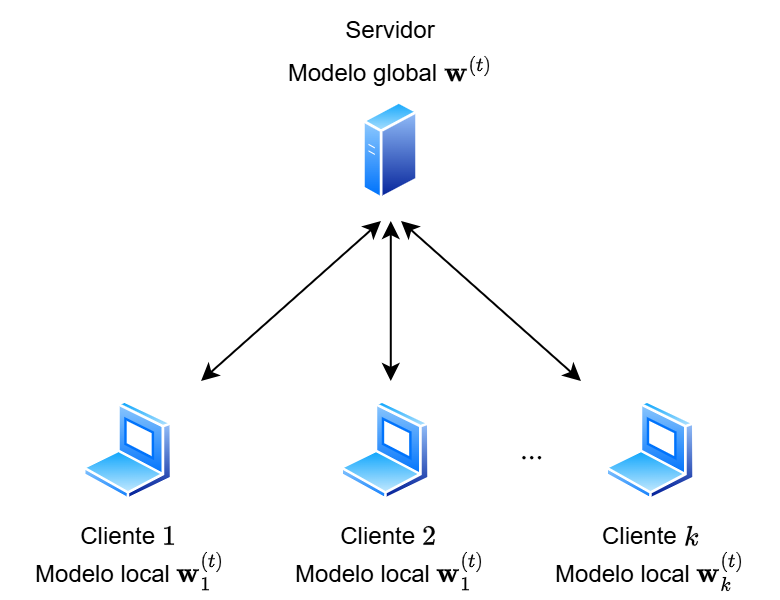
\includegraphics[width=0.8\textwidth]{./images/image1.png}
\caption{\label{fig:figure1}Ciclo de comunicación en aprendizaje federado.}
\end{center}
\end{figure}


\subsection{Proceso de optimización federada}

El objetivo del FL se puede formalizar como la minimización de una función de pérdida global
definida como el promedio ponderado de las pérdidas locales de cada cliente
\cite{DBLP:journals/corr/abs-1908-07873}:

\begin{equation}
  \min_{\mathbf{w}} F(\mathbf{w}) = \sum_{k=1}^{K} \frac{n_k}{n} F_k(\mathbf{w}),
  \label{eq:fedobj}
\end{equation}

donde $F_k(\mathbf{w}) = \frac{1}{n_k} \sum_{i \in \mathcal{D}_k} \ell(\mathbf{w}; x_i, y_i)$
es la función de pérdida local del cliente $k$ y $\ell$ es la función de pérdida por muestra
(por ejemplo, entropía cruzada para clasificación). En el caso ideal en que los datos de todos
los clientes siguen la misma distribución —condición IID—, el gradiente local $\nabla F_k
(\mathbf{w})$ es un estimado insesgado del gradiente global $\nabla F(\mathbf{w})$, y el
SGD distribuido converge a las mismas cotas que el SGD centralizado
\cite{li2020convergencefedavgnoniiddata}.

En la práctica, sin embargo, los datos federados raramente satisfacen la condición IID. Cuando
$\nabla F_k(\mathbf{w}) \neq \nabla F(\mathbf{w})$ para algún cliente $k$, los múltiples
pasos de SGD local producen una secuencia de parámetros que se aleja del óptimo global en la
dirección del óptimo local de $F_k$ \cite{DBLP:journals/corr/abs-1910-06378}. Al promediar
los parámetros locales al final de cada ronda, el modelo global resultante puede encontrarse
en una región de alta pérdida para todos los participantes, degradando la calidad del modelo
y ralentizando la convergencia. Este fenómeno, conocido como \textit{client drift}, es el
objeto de estudio central de la presente investigación y se formaliza en detalle en la
Sección~\ref{sec:clientdrift}.

\subsection{Desafíos del aprendizaje federado}

El FL introduce un conjunto de desafíos técnicos que no existen o se manifiestan con menor
severidad en el aprendizaje centralizado \cite{DBLP:journals/corr/abs-1912-04977,
DBLP:journals/corr/abs-1908-07873}. En el contexto de esta investigación, el más relevante es
la \textit{heterogeneidad estadística}: la distribución de datos entre clientes —tanto en
etiquetas como en características— difiere de forma sistemática, introduciendo un sesgo en el
gradiente local que el algoritmo de agregación debe compensar para preservar la convergencia
global. Esta dimensión se desarrolla en detalle en la Sección~\ref{sec:heterogeneidad}.

Un segundo desafío es la \textit{heterogeneidad del sistema}: los clientes presentan capacidades
computacionales y de memoria heterogéneas, velocidades de comunicación variables y posibles
caídas o desconexiones durante el entrenamiento \cite{DBLP:journals/corr/abs-1908-07873}. En
escenarios \textit{cross-device}, este factor puede dominar el rendimiento del sistema; en el
escenario \textit{cross-silo} de esta investigación, se controla manteniendo todos los clientes
activos en cada ronda con hiperparámetros de entrenamiento idénticos.

La \textit{privacidad y seguridad} constituye el tercer desafío estructural del FL
\cite{DBLP:journals/corr/abs-1912-04977}. Aunque los datos locales no se transmiten
directamente, las actualizaciones de parámetros pueden filtrar información sobre los datos de
entrenamiento mediante ataques de inversión de gradiente o inferencia de membresía
\cite{DBLP:journals/corr/abs-1807-00459}. Si bien la presente investigación no aborda
mecanismos de privacidad diferencial ni agregación segura, la motivación del FL en el
dominio médico descansa precisamente sobre esta restricción.

Finalmente, la \textit{eficiencia de comunicación} es un desafío práctico significativo: en cada
ronda de comunicación se transmiten todos los parámetros del modelo, cuyo tamaño puede superar
los cientos de megabytes para modelos modernos de visión \cite{mahmud2026survey}. Las cuatro
arquitecturas estudiadas en esta investigación se seleccionaron, entre otros criterios, por operar
a escalas de parámetros comparables y manejables ($\sim$5--8M parámetros), lo que hace que el
costo de comunicación sea equivalente entre familias y no constituya una variable de confusión.

% ============================================================
% 2.2 HETEROGENEIDAD ESTADÍSTICA Y CLIENT DRIFT
% ============================================================
\section{Heterogeneidad Estadística y Client Drift}
\label{sec:heterogeneidad}

\subsection{Datos IID y non-IID en aprendizaje federado}

En el aprendizaje automático estándar se asume que las muestras de entrenamiento son generadas
de forma independiente e idénticamente distribuida (IID) a partir de una distribución global
$P(X, Y)$ \cite{seo2025understanding}. En el contexto federado, esta condición implica que
cada cliente $k$ posee un subconjunto $\mathcal{D}_k$ muestreado de esa misma distribución
global, de modo que la distribución marginal de etiquetas y características es homogénea entre
participantes: $P_k(X, Y) \approx P(X, Y)$ para todo $k$.

En la práctica, los conjuntos de datos federados reales son no-IID (\textit{non-Independent and
Identically Distributed}): la distribución local $P_k(X, Y)$ varía entre clientes debido a
diferencias en las poblaciones atendidas, los protocolos de adquisición, los equipos utilizados
o los criterios de etiquetado \cite{g2024noniiddatafederatedlearning, seo2025understanding}.
Esta heterogeneidad tiene consecuencias directas sobre el proceso de optimización: si
$P_k(X, Y) \neq P_j(X, Y)$ para $k \neq j$, entonces $\nabla F_k(\mathbf{w}) \neq
\nabla F_j(\mathbf{w})$, y el gradiente promediado $\sum_k \frac{n_k}{n} \nabla F_k(\mathbf{w})$
puede apuntar en una dirección significativamente diferente al gradiente del óptimo global
$\nabla F(\mathbf{w})$ \cite{li2020convergencefedavgnoniiddata}. Li et al.\
\cite{li2020convergencefedavgnoniiddata} demostraron formalmente que, bajo condiciones non-IID,
FedAvg puede divergir o converger a un punto subóptimo distante del mínimo centralizado, con
una brecha de rendimiento que crece con el número de épocas locales $E$ y con el grado de
heterogeneidad entre los datos de los clientes.

\subsection{Taxonomía de la heterogeneidad}
\label{subsec:taxonomia}

Jiménez G. et al.\ \cite{g2024noniiddatafederatedlearning} proponen una taxonomía exhaustiva
de las formas en que los datos federados pueden diferir entre clientes. Las categorías
principales son:

\textbf{Sesgo de etiquetas} (\textit{label skew}): la distribución marginal de etiquetas
$P_k(Y)$ difiere entre clientes, mientras que la distribución condicional de características
dado la etiqueta $P_k(X \mid Y)$ puede ser homogénea. Es la forma más estudiada de
heterogeneidad y la que produce los efectos más severos sobre la convergencia
\cite{jimenez2503thorough}. En el contexto clínico, este sesgo es omnipresente: un hospital
especializado en oncología neurológica tendrá una proporción de tumores cerebrales muy
superior a la de un centro de atención primaria.

\textbf{Sesgo de características} (\textit{feature skew} o \textit{covariate shift}):
la distribución de entrada $P_k(X)$ varía entre clientes manteniendo constante la distribución
condicional $P_k(Y \mid X)$. Puede originarse en diferencias de equipamiento —distintos tipos
de escáneres MRI con protocolos de adquisición heterogéneos— o en variabilidad de iluminación,
resolución o preprocesamiento \cite{g2024noniiddatafederatedlearning}.

\textbf{Sesgo de cantidad} (\textit{quantity skew}): los clientes poseen volúmenes de datos
muy dispares, independientemente de la distribución de clases. Este desequilibrio afecta el
peso relativo de cada cliente en la agregación ponderada por $n_k / n$ y puede amplificar el
efecto del sesgo de etiquetas en los clientes con menos datos
\cite{g2024noniiddatafederatedlearning}.

\textbf{Heterogeneidad temporal}: la distribución de datos de un cliente varía a lo largo
del tiempo (\textit{concept drift}), lo que introduce inestabilidad adicional en el modelo
global \cite{DBLP:journals/corr/abs-1912-04977}.

La presente investigación opera exclusivamente sobre sesgo de etiquetas, controlado mediante
el parámetro de concentración $\alpha$ de la distribución de Dirichlet. Jiménez-Gutiérrez et al.\
\cite{jimenez2503thorough} han demostrado empíricamente que el sesgo de etiquetas produce
caídas de precisión de entre 10 y 40 puntos porcentuales sobre la línea base centralizada,
mientras que los sesgos de cantidad y características resultan prácticamente inocuos para
las arquitecturas estudiadas, lo que justifica la elección de este tipo de heterogeneidad
como variable experimental principal.

\subsection{Partición de Dirichlet para non-IID}

La distribución de Dirichlet $\text{Dir}(\alpha)$ es el mecanismo estándar para generar
particiones de datos con sesgo de etiquetas controlado en experimentos de FL
\cite{g2024noniiddatafederatedlearning, seo2025understanding}. Para un problema de
clasificación con $C$ clases y $K$ clientes, la partición se genera asignando a cada
cliente $k$ una proporción $\mathbf{q}_k = (q_{k,1}, \ldots, q_{k,C})$ muestreada de
$\text{Dir}(\alpha \cdot \mathbf{1}_C)$, donde $q_{k,c}$ es la fracción de muestras de la
clase $c$ asignadas al cliente $k$, satisfaciendo $\sum_k q_{k,c} = 1$ para toda clase $c$.

\sloppy El parámetro de concentración $\alpha > 0$ controla el grado de heterogeneidad: cuando
$\alpha \to 0$, cada cliente recibe datos de una única clase (heterogeneidad máxima); cuando
$\alpha \to \infty$, la partición converge a una distribución uniforme de clases (condición
IID) \cite{g2024noniiddatafederatedlearning}. La presente investigación emplea
$\alpha \in \{1000.0, 1.0, 0.3, 0.1, 0.03\}$, que cubren los regímenes de alta, media y baja heterogeneidad
respectivamente. A modo de referencia, Jiménez-Gutiérrez et al.\
\cite{jimenez2503thorough} reportan que los efectos críticos de degradación comienzan
a manifestarse de forma consistente para $\alpha \leq 0.5$ en las arquitecturas evaluadas.


\begin{figure} 
\begin{center}
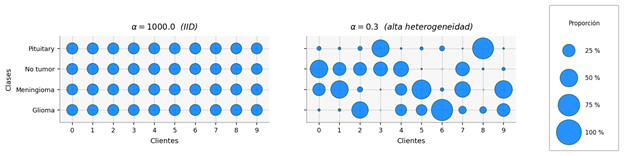
\includegraphics[width=\textwidth]{./images/image2.png}
\caption{\label{fig:figure2}Distribución de etiquetas por cliente bajo distintos valores de $\alpha$ — Brain Tumor MRI ($K=10$, semilla 42).}
\end{center}
\end{figure}

\subsection{Client drift: definición y mecanismo}
\label{sec:clientdrift}

El \textit{client drift} se define como la divergencia entre los parámetros del modelo de un
cliente al final de su entrenamiento local y el modelo global al inicio de esa misma ronda de
comunicación \cite{DBLP:journals/corr/abs-1910-06378}. Formalmente, dado que en la ronda $t$
el cliente $k$ recibe el modelo global $\mathbf{w}^{(t)}$ y realiza $E$ épocas de SGD local,
obteniendo $\mathbf{w}_k^{(t)}$, el vector de deriva del cliente $k$ se define como:

\begin{equation}
  \boldsymbol{\delta}_k^{(t)} = \mathbf{w}_k^{(t)} - \mathbf{w}^{(t)},
  \label{eq:drift}
\end{equation}

denominado en la literatura como \textit{pseudo-gradiente} \cite{DBLP:journals/corr/abs-1910-06378}.
El cliente drift es, por tanto, el efecto acumulado de múltiples pasos de SGD en la dirección
del óptimo local $\mathbf{w}_k^*$ en lugar del óptimo global $\mathbf{w}^*$.

El mecanismo causal del drift opera en tres niveles. En primer lugar, bajo condiciones non-IID,
el gradiente local $\nabla F_k(\mathbf{w})$ es un estimado sesgado del gradiente global
$\nabla F(\mathbf{w})$: existe una diferencia sistemática $\nabla F_k(\mathbf{w}) -
\nabla F(\mathbf{w}) \neq \mathbf{0}$ que depende de cuán diferente es $P_k(X,Y)$ respecto
a $P(X,Y)$ \cite{DBLP:journals/corr/abs-1910-06378}. En segundo lugar, este sesgo se amplifica
con cada paso adicional de SGD local: después de $E$ épocas, el modelo local se ha alejado de
$\mathbf{w}^{(t)}$ en la dirección del gradiente sesgado, acumulando una deriva proporcional
a $E$ y a la tasa de aprendizaje $\eta$ \cite{li2020convergencefedavgnoniiddata}. En tercer
lugar, al agregar los pseudo-gradientes $\boldsymbol{\delta}_k^{(t)}$ de múltiples clientes con
distribuciones distintas, el modelo global $\mathbf{w}^{(t+1)} = \mathbf{w}^{(t)} +
\sum_k \frac{n_k}{n} \boldsymbol{\delta}_k^{(t)}$ puede converger hacia un punto que minimiza
un promedio de funciones con óptimos en direcciones contradictorias, resultando en un modelo
subóptimo para todos los participantes \cite{DBLP:journals/corr/abs-1910-06378}.

Una observación fundamental para la presente investigación es que el drift no se distribuye
uniformemente entre las capas del modelo: trabajos como los de Son et al.\
\cite{son2022comparisons} han demostrado empíricamente que las capas de clasificación y de
normalización exhiben drift de mayor magnitud que las capas de extracción de características de
bajo nivel, y que esta distribución varía entre arquitecturas. Es precisamente esta estructura
interna del drift la que esta investigación busca caracterizar.




\begin{figure}[ht]
\centering
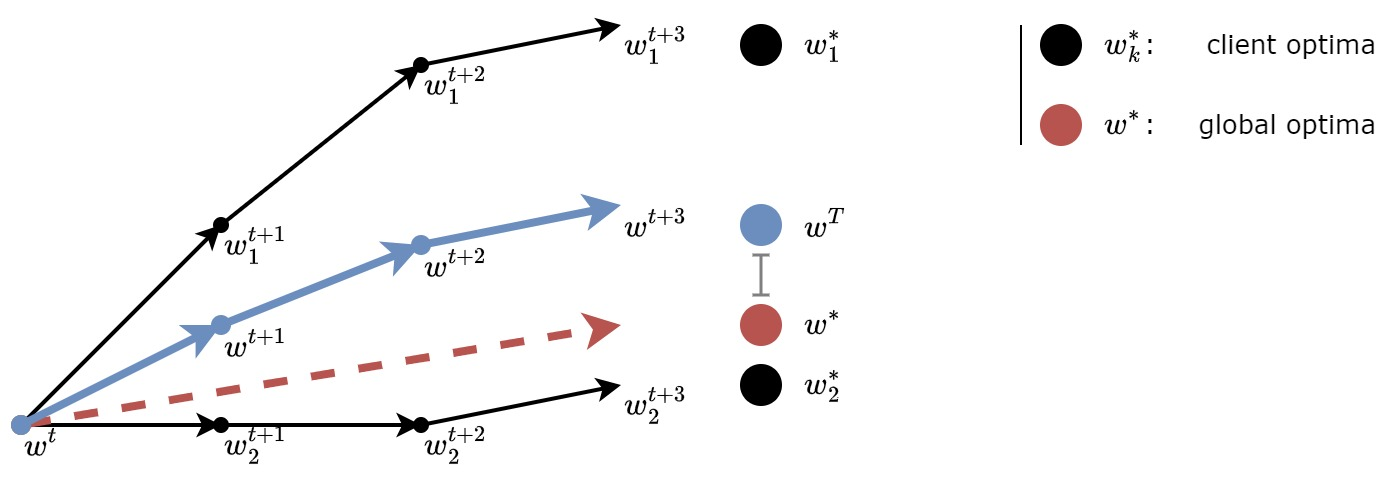
\includegraphics[width=\textwidth]{./images/image3.png}
\caption{Mecanismo del client drift en el espacio de parámetros.}
\label{fig:figure3}

\vspace{0.2cm}
\small Fuente: Obtenido de Le et al. (2024) \cite {le2024exploring}.
\end{figure}

\subsection{Impacto del drift sobre la convergencia}

Li et al.\ \cite{li2020convergencefedavgnoniiddata} demostraron que la cota de convergencia de
FedAvg bajo condiciones non-IID incluye un término adicional proporcional a la \textit{gradient
diversity}, definida como la discrepancia esperada entre los gradientes locales y el gradiente
global:

\begin{equation}
  \Gamma = F^* - \sum_{k=1}^{K} \frac{n_k}{n} F_k^*,
  \label{eq:diversity}
\end{equation}

donde $F^* = \min_{\mathbf{w}} F(\mathbf{w})$ es el óptimo global y $F_k^*$ es el óptimo
local del cliente $k$. Cuando los datos son IID, $\Gamma = 0$ y la cota de convergencia se
reduce a la del SGD centralizado. Bajo non-IID, $\Gamma > 0$ y actúa como un sesgo permanente
que no desaparece con el aumento del número de rondas de comunicación $T$
\cite{li2020convergencefedavgnoniiddata}. Este resultado teórico establece que la magnitud del drift, y por tanto de la degradación del rendimiento, depende directamente del grado de
heterogeneidad de los datos entre clientes, cuantificado en esta investigación mediante el
parámetro $\alpha$ de la distribución de Dirichlet.

Desde la perspectiva empírica, Karimireddy et al.\ \cite{DBLP:journals/corr/abs-1910-06378}
mostraron que FedAvg puede exhibir inestabilidad de convergencia incluso con tasas de
aprendizaje moderadas bajo alta heterogeneidad ($\alpha \to 0$), y que el número óptimo de
épocas locales $E$ decrece con el grado de no-IID. Esta dinámica es relevante para interpretar
los perfiles de drift registrados en el Capítulo de Análisis: una mayor oscilación de la curva
de accuracy a lo largo de las rondas es un indicador indirecto de un alto nivel de drift
acumulado.

% ============================================================
% 2.3 ALGORITMOS DE OPTIMIZACIÓN FEDERADA
% ============================================================
\section{Algoritmos de Optimización Federada}

\subsection{FedAvg}

El algoritmo FedAvg (\textit{Federated Averaging}), propuesto por McMahan et al.\
\cite{DBLP:journals/corr/McMahanMRA16}, constituye el método de referencia del aprendizaje
federado moderno. Su procedimiento es el siguiente: en cada ronda de comunicación $t$, el
servidor selecciona un subconjunto de $m$ clientes (o la totalidad de ellos en escenarios
\textit{cross-silo}), les envía el modelo global actual $\mathbf{w}^{(t)}$, cada cliente
realiza $E$ épocas de SGD local con tasa de aprendizaje $\eta$ sobre su conjunto de datos
$\mathcal{D}_k$, y el servidor agrega los modelos resultantes mediante un promedio ponderado
por tamaño de dataset:

\begin{equation}
  \mathbf{w}^{(t+1)} = \sum_{k=1}^{K} \frac{n_k}{n} \mathbf{w}_k^{(t)}.
  \label{eq:fedavg}
\end{equation}

La simplicidad algorítmica de FedAvg es su principal virtud: no requiere comunicación adicional
entre clientes, no introduce hiperparámetros dependientes de la arquitectura y se implementa
con cambios mínimos sobre cualquier bucle de entrenamiento estándar. Sin embargo, como se
mostró en la sección anterior, el promedio de parámetros locales entrenados sobre datos
heterogéneos puede producir un modelo global subóptimo \cite{li2020convergencefedavgnoniiddata}.
En esta investigación, FedAvg se emplea como algoritmo de referencia para caracterizar el
perfil de drift sin la intervención de mecanismos de corrección.

\subsection{FedProx}

\sloppy FedProx \cite{DBLP:journals/corr/abs-1812-06127}, propuesto por Sahu et al., extiende FedAvg
añadiendo un término de regularización proximal a la función de pérdida local de cada cliente:

\begin{equation}
  h_k(\mathbf{w}; \mathbf{w}^{(t)}) = F_k(\mathbf{w}) + \frac{\mu}{2}
  \|\mathbf{w} - \mathbf{w}^{(t)}\|^2,
  \label{eq:fedprox}
\end{equation}

donde $\mu \geq 0$ es el hiperparámetro de regularización proximal. El término
$\frac{\mu}{2}\|\mathbf{w} - \mathbf{w}^{(t)}\|^2$ penaliza el alejamiento del modelo
local respecto al modelo global recibido al inicio de la ronda, actuando como una restricción
suave que limita la magnitud del drift $\|\boldsymbol{\delta}_k^{(t)}\|$. Cuando $\mu = 0$,
FedProx se reduce a FedAvg. Al aumentar $\mu$, el modelo local se mantiene más cercano al
modelo global, lo que reduce el drift a costa de introducir un sesgo de regularización que
puede ralentizar la convergencia cuando los datos locales contienen información específica
valiosa \cite{DBLP:journals/corr/abs-1812-06127}.

Sahu et al.\ \cite{DBLP:journals/corr/abs-1812-06127} demostraron que FedProx converge bajo
condiciones de heterogeneidad estadística y de sistema donde FedAvg puede divergir, y que el
término proximal produce una mejora en la estabilidad del modelo global particularmente visible
bajo alta heterogeneidad. En esta investigación, FedProx se emplea con el objetivo de
evaluar si la reducción del drift producida por la regularización proximal interactúa de forma
diferente con las cuatro familias arquitectónicas, o si su efecto es homogéneo entre ellas.

\subsection{SCAFFOLD}

SCAFFOLD (\textit{Stochastic Controlled Averaging for Federated Learning}),
propuesto por Karimireddy et al.\ \cite{DBLP:journals/corr/abs-1910-06378}, introduce la
formalización más rigurosa del client drift al tiempo que propone su corrección mediante
variables de control de varianza. Cada cliente $k$ mantiene una variable de control
$\mathbf{c}_k$ que estima el gradiente local esperado, y el servidor mantiene $\mathbf{c}$
como estimado del gradiente global. La actualización de SGD local corregida por SCAFFOLD es:

\begin{equation}
  \mathbf{w}_k \leftarrow \mathbf{w}_k - \eta \left( \nabla F_k(\mathbf{w}_k)
  - \mathbf{c}_k + \mathbf{c} \right),
  \label{eq:scaffold}
\end{equation}

donde el término $-\mathbf{c}_k + \mathbf{c}$ actúa como una corrección de varianza que
compensa la diferencia entre el gradiente local y el global. Al final de cada ronda, las
variables de control se actualizan utilizando la diferencia entre las posiciones de los
parámetros antes y después del entrenamiento local. Karimireddy et al.\
\cite{DBLP:journals/corr/abs-1910-06378} demostraron que SCAFFOLD converge bajo condiciones
non-IID independientemente del número de épocas locales $E$ —propiedad que FedAvg no satisface
para $E > 1$ en escenarios heterogéneos.

SCAFFOLD no se emplea directamente como algoritmo experimental en esta investigación, pero su
marco teórico es central: la noción de pseudo-gradiente $\boldsymbol{\delta}_k^{(t)}$ definida
en la ecuación \eqref{eq:drift} proviene de este trabajo, y la corrección de varianza de
SCAFFOLD puede interpretarse como la operación inversa a la acumulación de drift. Comprender
SCAFFOLD es, por tanto, una condición necesaria para interpretar con precisión las métricas de
drift registradas en los experimentos.

% ============================================================
% 2.4 ARQUITECTURAS DE VISIÓN POR COMPUTADORA
% ============================================================
\section{Arquitecturas de Visión por Computadora}

Las cuatro familias arquitectónicas estudiadas en esta investigación —redes neuronales
convolucionales (CNNs), Vision Transformers (ViTs), State-Space Models (SSMs) y Vision Graph
Neural Networks (Vision GNNs)— procesan la información visual mediante mecanismos distintos. Estas diferencias estructurales se denominan \textit{sesgos
inductivos} (\textit{inductive biases}): suposiciones implícitas sobre la estructura de los
datos que determinan qué tipo de patrones puede aprender cada arquitectura de forma eficiente
\cite{xu2023fedconv}. Como se argumentará a lo largo de esta sección, los sesgos inductivos de
cada familia tienen implicaciones directas sobre su comportamiento bajo optimización federada
con datos heterogéneos, dado que determinan cómo los parámetros del modelo responden a las
distribuciones locales de cada cliente.


\begin{figure} 
\begin{center}
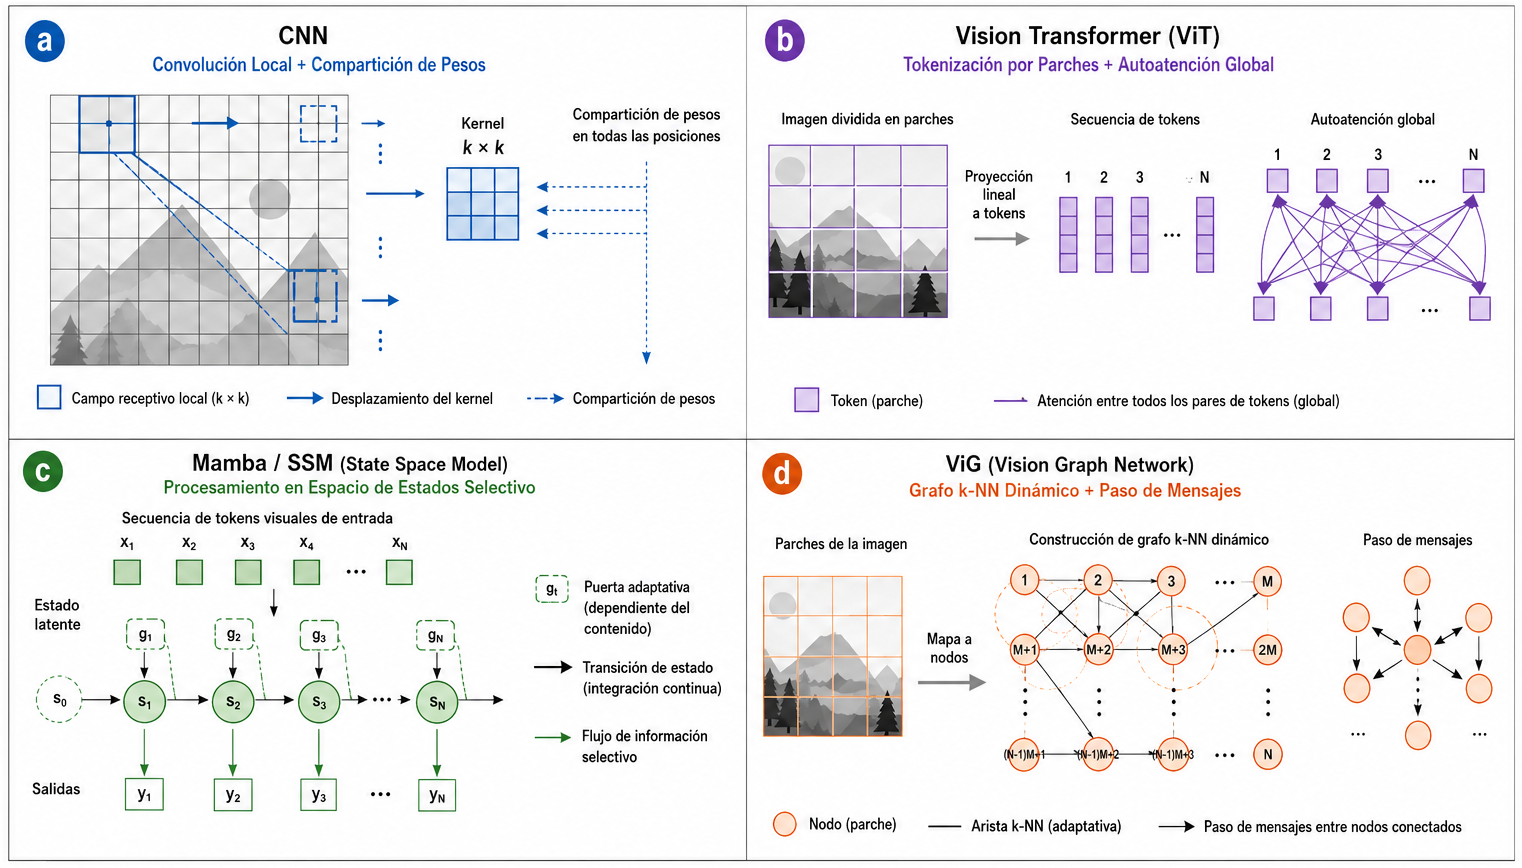
\includegraphics[width=\textwidth]{./images/image4.png}
\caption{\label{fig:figure4}Comparación de los sesgos inductivos en cuatro familias de arquitecturas de visión por computador.}
\end{center}
\end{figure}

\subsection{Redes Neuronales Convolucionales}

\subsubsection{Principios y sesgos inductivos}

Las redes neuronales convolucionales procesan la información visual mediante la operación de
convolución discreta \cite{heaton2018ian}. Dado
un mapa de activación de entrada $\mathbf{X} \in \mathbb{R}^{H \times W \times C_{in}}$, una
capa convolucional aplica un conjunto de filtros $\mathbf{F} \in \mathbb{R}^{k \times k \times
C_{in} \times C_{out}}$ de tamaño $k \times k$, donde cada filtro recorre la imagen de forma
deslizante produciendo un mapa de respuesta de dimensiones reducidas. El parámetro compartido
más importante es el filtro en sí: el mismo conjunto de pesos $\mathbf{F}$ se aplica en todas
las posiciones espaciales de la imagen (\textit{weight sharing}), lo que confiere a las CNNs
el sesgo inductivo de \textit{equivarianza traslacional}: si un patrón se desplaza en la imagen,
su representación se desplaza de forma correspondiente en el mapa de activación
\cite{xu2023fedconv}.

Los sesgos inductivos de la CNN son tres: (1) \textit{localidad espacial}, dado que cada
neurona de salida depende únicamente de una región $k \times k$ de la entrada;
(2) \textit{equivarianza traslacional}, consecuencia directa del weight sharing; y
(3) \textit{jerarquía de características}, donde las capas iniciales aprenden detectores de
bordes y texturas de bajo nivel, y las capas profundas combinan estos detectores para
representar objetos complejos \cite{pieri2023handlingdataheterogeneityarchitectural}.

En el contexto federado, la localidad espacial implica que los filtros convolucionales aprenden
patrones visuales locales que son altamente dependientes de las clases presentes en los datos de
entrenamiento de cada cliente. Bajo sesgo de etiquetas severo ($\alpha = 0.1$), los filtros de
distintos clientes pueden especializarse en detectar características propias de las clases
locales, dando lugar a representaciones locales incompatibles que producen un alto drift al ser
promediadas \cite{qu2022rethinking}.


\begin{figure}
\begin{center}
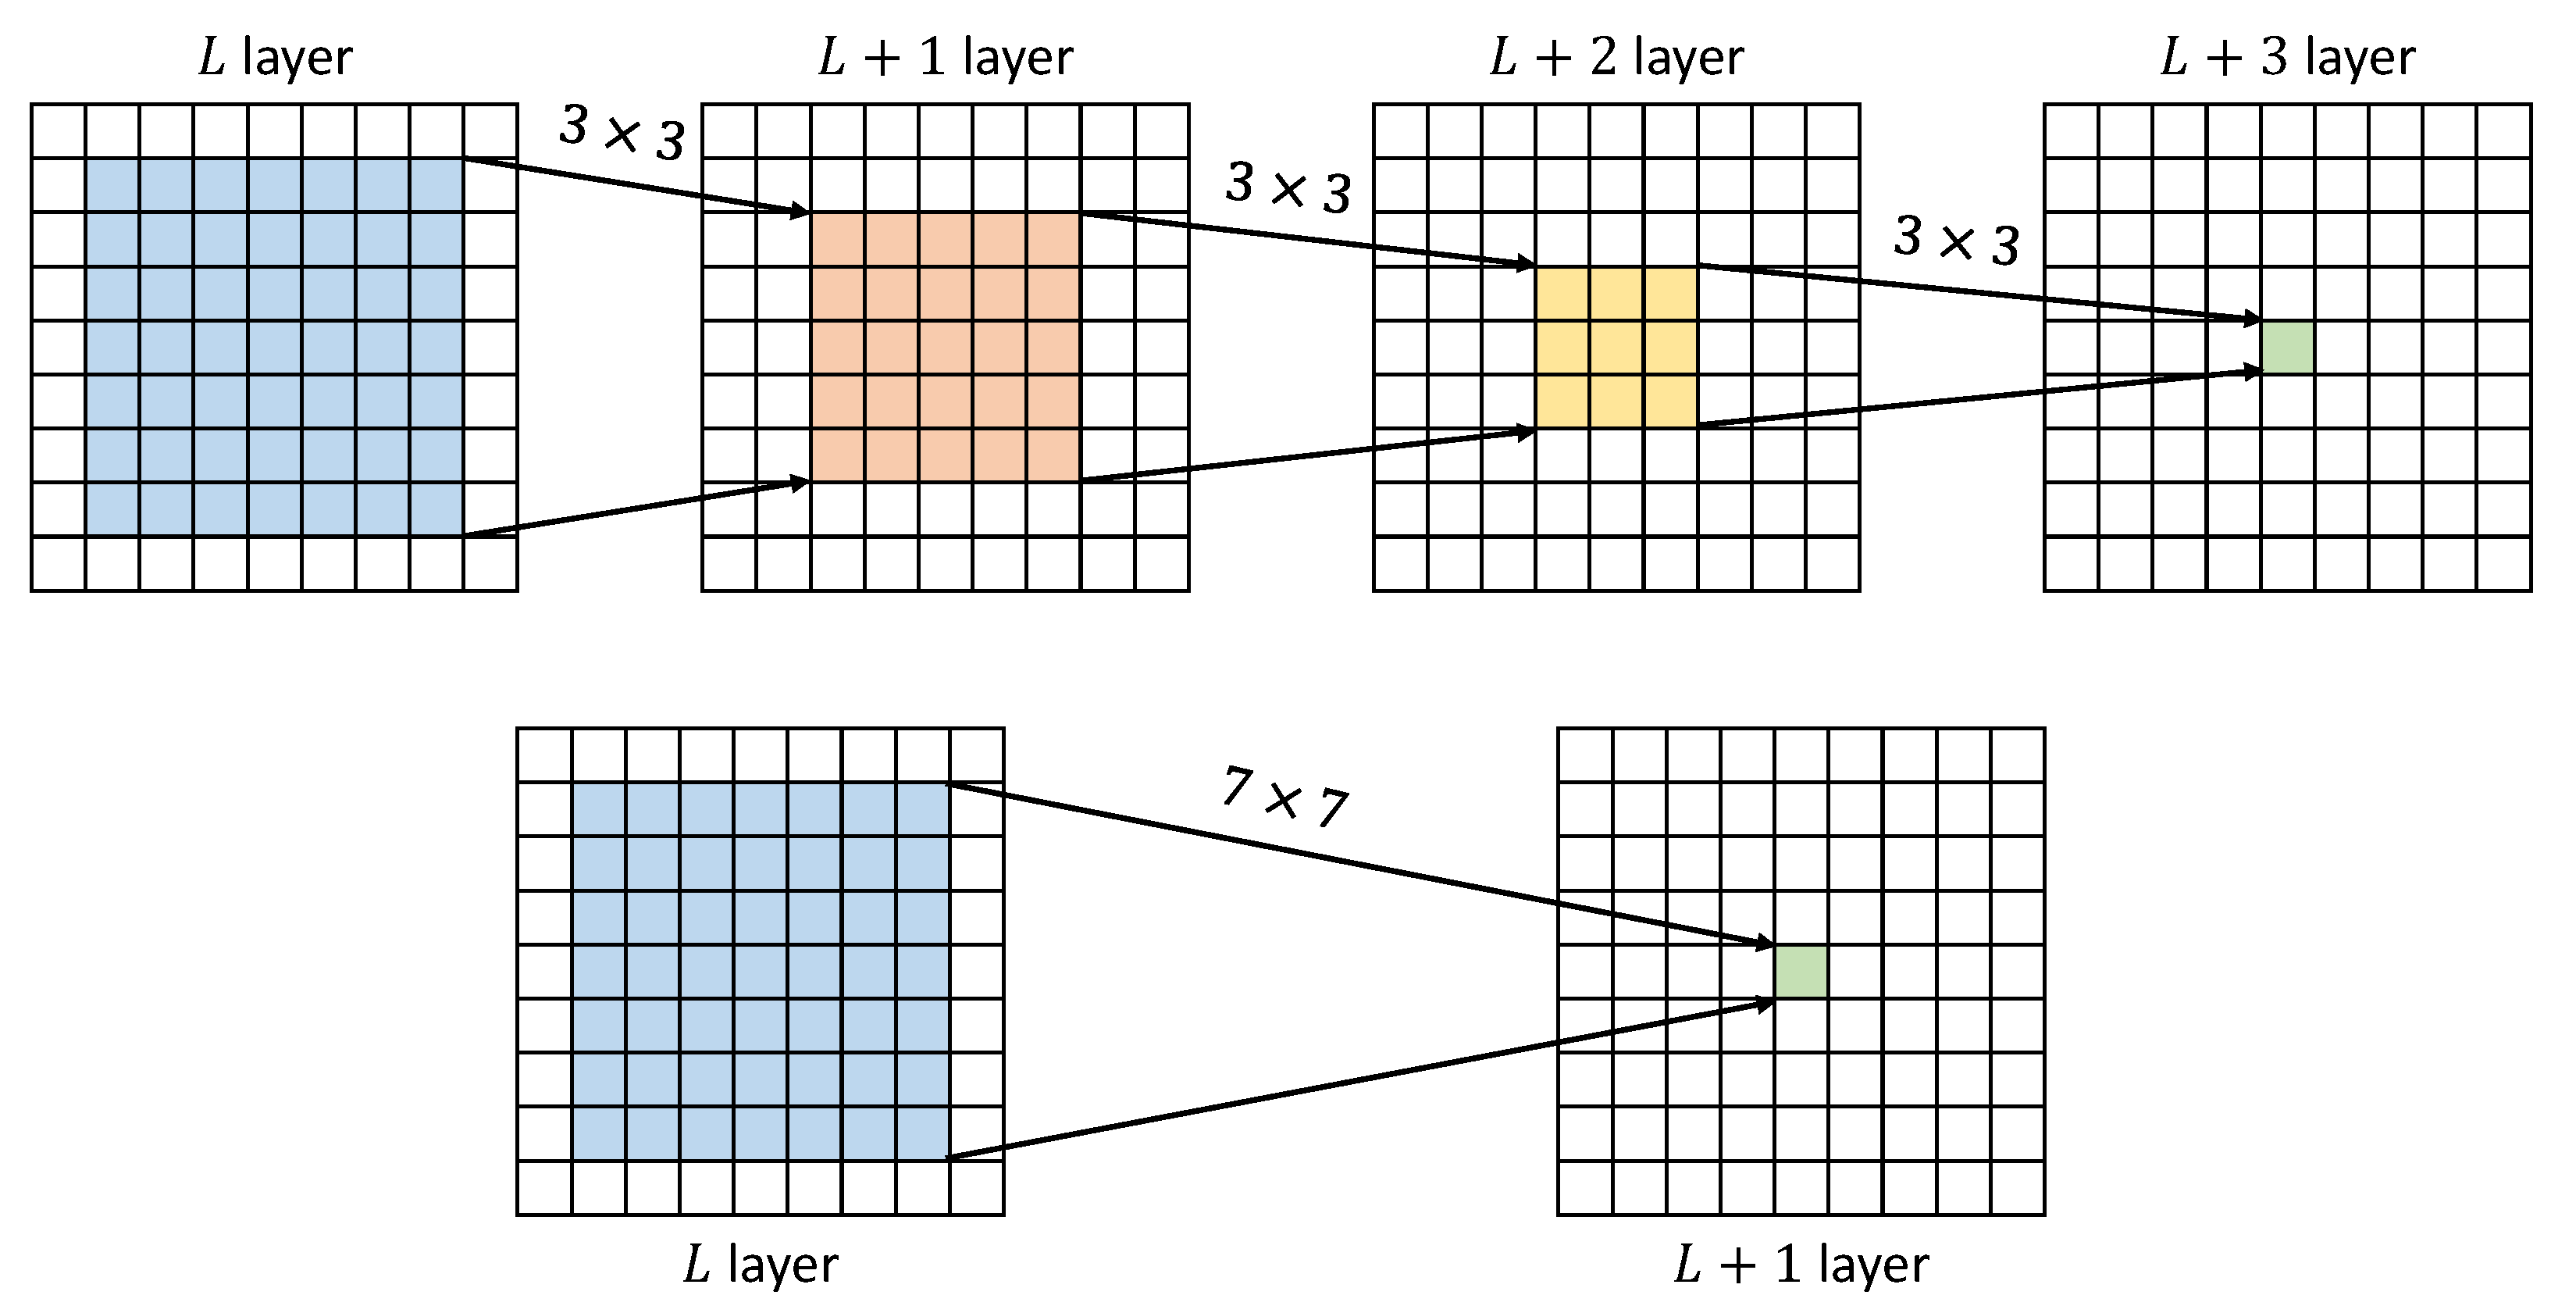
\includegraphics[width=\textwidth]{./images/image5.png}
\caption{\label{fig:figure5} Convolución discreta de un filtro \textit{$3\times3$} sobre un mapa de activación. Una pila de tres capas convolucionales de \textit{$3\times3$} tiene un campo receptivo efectivo de \textit{$7\times7$}.}

\vspace{0.2cm}
\small Fuente: Obtenido de Dong et al. (2023) \cite{app13063403}.

\end{center}
\end{figure}

\subsubsection{EfficientNet-B1 y la familia EfficientNet}

EfficientNet \cite{DBLP:journals/corr/abs-1905-11946} es una familia de
redes neuronales convolucionales diseñada mediante escalado compuesto (\textit{compound
scaling}): en lugar de escalar únicamente la profundidad, la anchura o la resolución de la red
de forma independiente, EfficientNet escala las tres dimensiones simultáneamente siguiendo
coeficientes determinados por búsqueda de arquitectura neural (NAS). EfficientNet-B1 es una de las variantes de menor tamaño de la familia, con aproximadamente 5.3 millones de parámetros y una
resolución de entrada estándar de $224 \times 224$ píxeles.

El bloque constructivo de EfficientNet es el \textit{MBConv} (\textit{Mobile Inverted
Bottleneck Convolution}), que combina una convolución puntual de expansión, una convolución
\textit{depthwise} separable y un módulo de \textit{Squeeze-and-Excitation} (SE) que recalibra
los mapas de canales mediante atención de canal global. Esta combinación hace a EfficientNet
computacionalmente eficiente al reducir el número de parámetros respecto a las redes totalmente
densas, mientras que el módulo SE introduce una forma limitada de contexto global dentro de
cada bloque, aunque sin llegar a la atención global de los ViTs
\cite{pieri2023handlingdataheterogeneityarchitectural}.

EfficientNet-B1 es el representante CNN elegido en esta investigación por tres razones: (1) su
escala de parámetros es comparable con ViT-Tiny y Vim-Tiny, eliminando el tamaño del modelo
como variable de confusión; (2) ha sido ampliamente utilizado en benchmarks de imagenología
médica, incluida la clasificación de tumores cerebrales \cite{chenfederated}; y (3) su
dependencia de Batch Normalization lo convierte en el candidato natural para la ablación de
normalización descrita en la Sección \ref{subsec:normalizacion}.

\begin{figure} 
\begin{center}
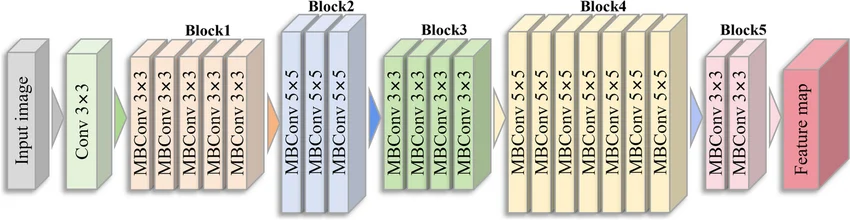
\includegraphics[width=\textwidth]{./images/image6.png}
\caption{\label{fig:figure6}Arquitectura EfficientNet-B1.}
\vspace{0.2cm}
\small Fuente: Obtenido de Dai et al. (2025) \cite {dai2025image}.

\end{center}
\end{figure}

\subsubsection{Batch Normalization y su interacción con FL}

Batch Normalization (BN) \cite{DBLP:journals/corr/IoffeS15} es una técnica de normalización que estandariza las activaciones de cada capa
usando las estadísticas del mini-batch actual. Para una activación $x$ en el mini-batch
$\mathcal{B} = \{x_1, \ldots, x_m\}$:

\begin{equation}
  \text{BN}(x) = \gamma \cdot \frac{x - \hat{\mu}_{\mathcal{B}}}
  {\sqrt{\hat{\sigma}^2_{\mathcal{B}} + \varepsilon}} + \beta,
  \label{eq:bn}
\end{equation}

donde $\hat{\mu}_{\mathcal{B}} = \frac{1}{m}\sum_{i=1}^m x_i$ y
$\hat{\sigma}^2_{\mathcal{B}} = \frac{1}{m}\sum_{i=1}^m (x_i - \hat{\mu}_{\mathcal{B}})^2$
son la media y varianza del mini-batch, y $\gamma$, $\beta$ son parámetros aprendibles de
escala y desplazamiento. Adicionalmente, BN mantiene estadísticas móviles (\textit{running
mean} y \textit{running variance}) que se actualizan durante el entrenamiento y se utilizan
durante la inferencia.

En el entorno federado con datos non-IID, BN introduce una vulnerabilidad específica que ha
sido formalizada por Wang et al.\ \cite{wang2023batch}: dado que cada cliente computa
$\hat{\mu}_{\mathcal{B}}^{(k)}$ y $\left(\hat{\sigma}^{2}_{\mathcal{B}}\right)^{(k)}$ sobre mini-batches
muestreados de su distribución local $P_k(X)$, las estadísticas resultantes son estimados
sesgados de las estadísticas globales $\mu$ y $\sigma^2$ de la distribución global $P(X)$.
Este sesgo tiene dos consecuencias sobre el modelo global producido por FedAvg. Primero, un
\textit{desajuste en el forward pass}: cuando los parámetros aprendibles $\gamma$, $\beta$
son promediados entre clientes, el modelo global hereda una normalización calibrada para
estadísticas locales inconsistentes entre sí, corrompiendo las representaciones intermedias
para todas las muestras \cite{wang2023batch}. Segundo, un \textit{desajuste en el backward
pass}: los gradientes respecto a $\gamma$ y $\beta$ se calculan usando las estadísticas locales
de cada cliente, de modo que las actualizaciones de estos parámetros apuntan en direcciones
distintas para clientes con distribuciones heterogéneas, amplificando el drift en las capas
de normalización \cite{du2022rethinking}.

Wang et al.\ \cite{wang2023batch} demostraron analíticamente que este sesgo de gradiente
inducido por BN es proporcional a la discrepancia entre las estadísticas locales y globales,
y que su magnitud crece con el grado de heterogeneidad. Du et al.\ \cite{du2022rethinking}
confirmaron empíricamente que la sustitución de BN por estrategias de normalización
independientes del batch —Layer Normalization o Group Normalization— reduce de forma
consistente la degradación del rendimiento bajo condiciones non-IID.

\subsection{Vision Transformers}

\subsubsection{Mecanismo de autoatención y tokenización}

Los Vision Transformers (ViT) \cite{DBLP:journals/corr/abs-2010-11929} adaptan la arquitectura
Transformer, originalmente desarrollada para procesamiento de lenguaje natural, al dominio de
la visión por computadora mediante un proceso de tokenización de la imagen. Dada una imagen
de entrada $\mathbf{I} \in \mathbb{R}^{H \times W \times C}$, se divide en $N = \frac{HW}{P^2}$
parches no solapados de tamaño $P \times P$ píxeles. Cada parche se aplana y se proyecta
linealmente a un vector de dimensión $d$, produciendo una secuencia de tokens
$\mathbf{Z} = [\mathbf{z}_1, \ldots, \mathbf{z}_N] \in \mathbb{R}^{N \times d}$. Se añade
un token de clasificación \texttt{[CLS]} y codificaciones posicionales para preservar
información espacial.

El bloque central de los ViTs es el mecanismo de \textit{Multi-Head Self-Attention} (MHSA).
Para un conjunto de tokens $\mathbf{Z}$, las matrices de consulta $\mathbf{Q}$, clave
$\mathbf{K}$ y valor $\mathbf{V}$ se obtienen mediante proyecciones lineales:

\begin{equation}
  \text{Attention}(\mathbf{Q}, \mathbf{K}, \mathbf{V}) =
  \text{softmax}\!\left(\frac{\mathbf{Q}\mathbf{K}^\top}{\sqrt{d_k}}\right)\mathbf{V},
  \label{eq:attention}
\end{equation}

donde $d_k$ es la dimensión de las cabezas de atención. La propiedad clave de este mecanismo
es que cada token puede atender simultáneamente a todos los demás tokens de la secuencia,
estableciendo dependencias globales desde la primera capa sin ninguna restricción de localidad
espacial \cite{qu2022rethinking}. Este sesgo inductivo —la capacidad de capturar contexto
global— contrasta fundamentalmente con la localidad de las CNNs.

En el contexto federado, la ausencia de dependencia de estadísticas de mini-batch hace que el
mecanismo de atención no sufra el desajuste de normalización identificado para las CNNs con BN.
La variabilidad entre clientes se manifiesta en cambio en los patrones de atención aprendidos
—las matrices $\mathbf{Q}$, $\mathbf{K}$, $\mathbf{V}$— que pueden especializarse en las
relaciones entre regiones de imagen propias de las clases locales de cada cliente
\cite{qu2022rethinking, pieri2023handlingdataheterogeneityarchitectural}.



\begin{figure}[ht]
\centering
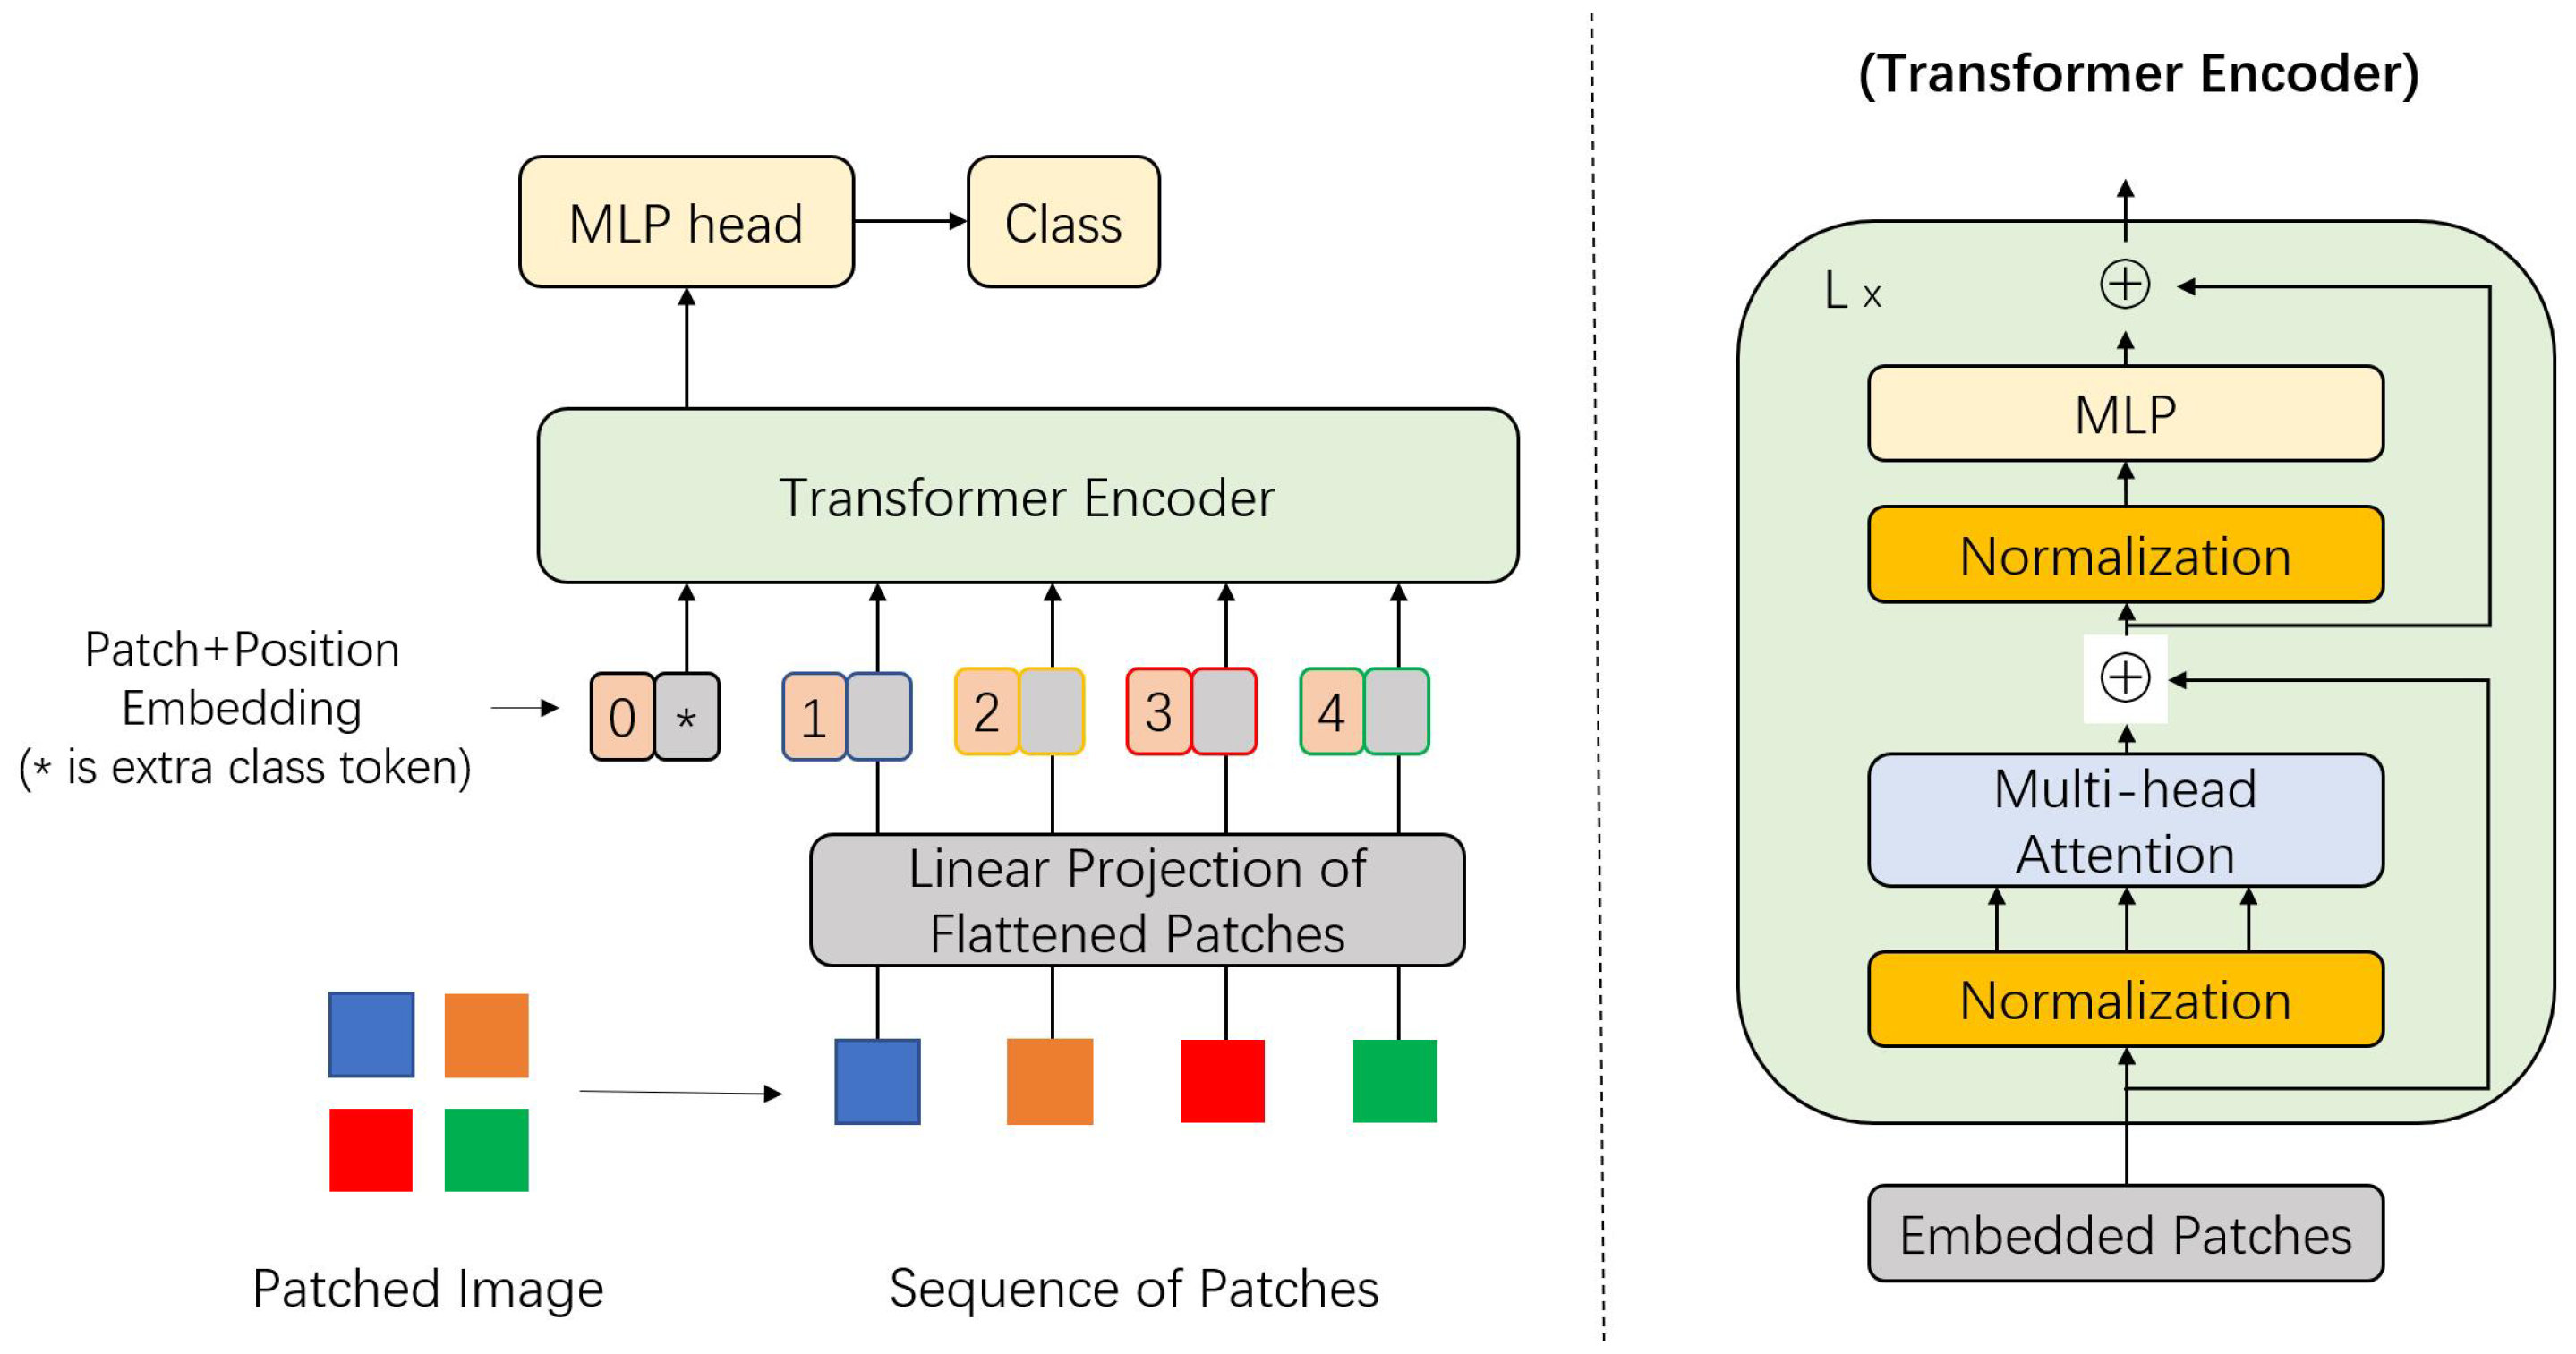
\includegraphics[width=\textwidth]{./images/image7.png}
\caption{Arquitectura de Vision Transformer.}
\label{fig:figure7}

\vspace{0.2cm}
\small Fuente: Obtenido de Wang et al. (2025) \cite{wang2025vision}.
\end{figure}



\subsubsection{ViT-Tiny}

El modelo empleado en esta investigación es \texttt{vit\_tiny\_patch16\_224}, cargado mediante
la librería \texttt{timm}. Esta variante usa parches de $16 \times 16$ píxeles sobre imágenes
de $224 \times 224$, generando $N = 196$ tokens. La dimensión de embedding es $d = 192$, con 3
cabezas de atención y 12 bloques Transformer, resultando en aproximadamente 5.7 millones de
parámetros. LayerNorm \cite{ba2016layernormalization} se aplica de forma nativa antes de cada bloque de atención y antes
de cada bloque MLP (\textit{pre-norm}), en contraste con la arquitectura original de Transformer
que usaba \textit{post-norm}.

ViT-Tiny se selecciona como representante de la familia ViT por ser la variante de menor costo
computacional con rendimiento competitivo en clasificación de imágenes, y por su escala de
parámetros comparable con EfficientNet-B1 y Vim-Tiny, lo que garantiza una comparación
arquitectónica justa. Su uso de LayerNorm nativo lo ubica, desde la perspectiva de la
normalización, en el extremo opuesto a EfficientNet-B1 con BN, siendo el modelo de referencia
para la estabilidad federada esperada según la literatura
\cite{wang2023batch, casella2023experimentingnormalizationlayersfederated}.


\begin{figure}[ht]
\centering
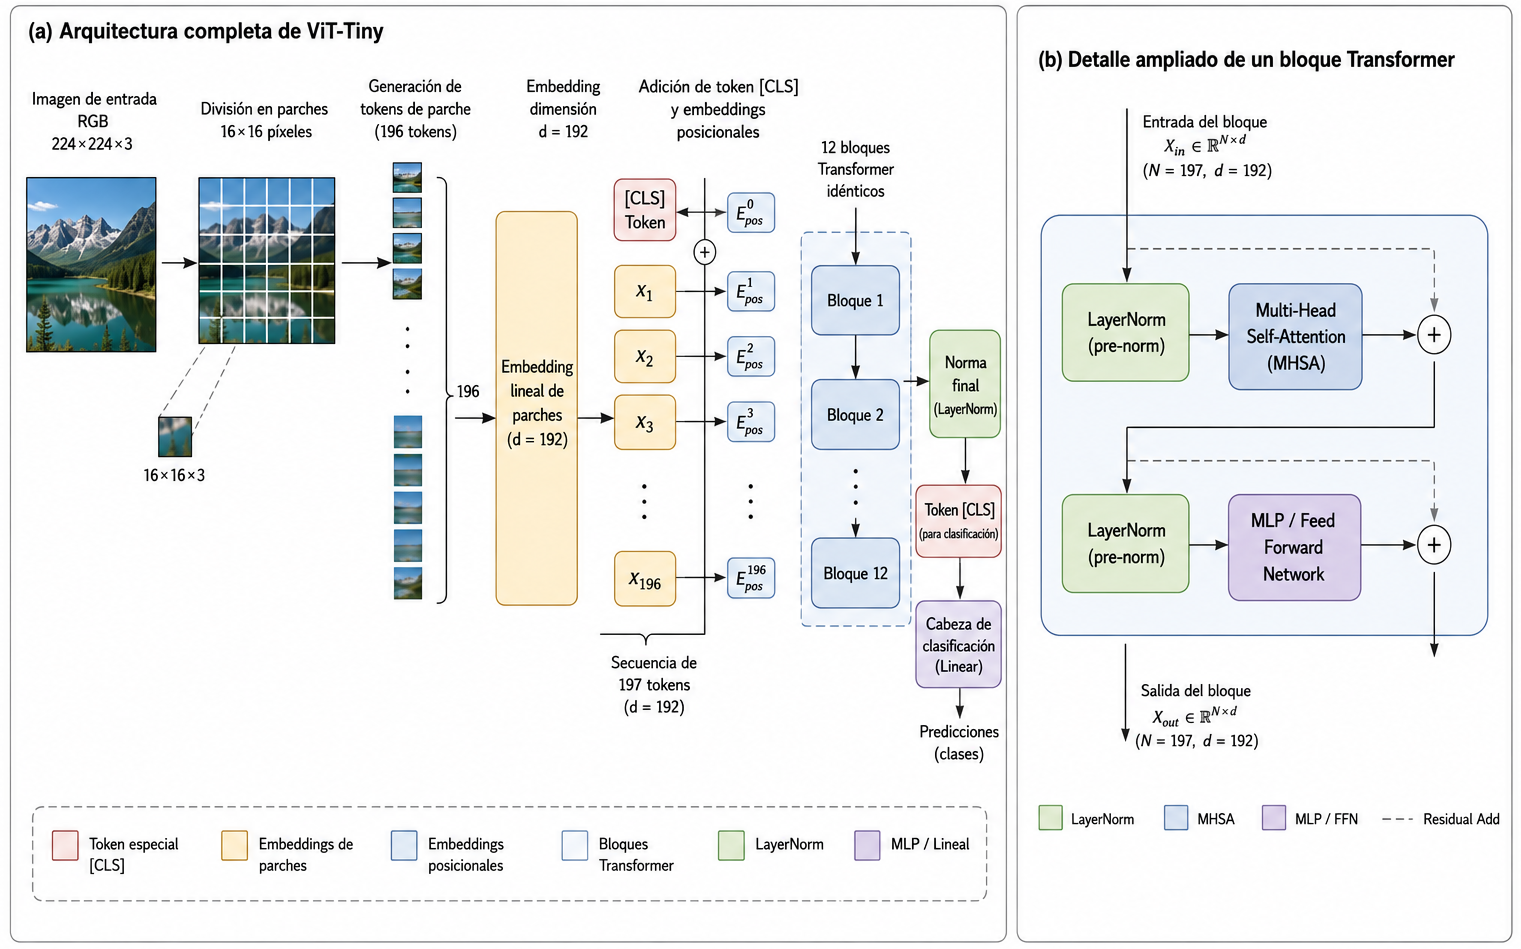
\includegraphics[width=\textwidth]{./images/image8.png}
\caption{Estructura completa de ViT-Tiny (\texttt{vit\_tiny\_patch16\_224})}
\label{fig:figure8}


\end{figure}


\subsubsection{Layer Normalization}

Layer Normalization (LN) \cite{ba2016layernormalization}
normaliza las activaciones a lo largo de la dimensión de características de una única muestra,
en lugar de a lo largo de la dimensión del batch como hace BN. Para una activación
$\mathbf{x} \in \mathbb{R}^d$ de una muestra individual:

\begin{equation}
  \text{LN}(\mathbf{x}) = \gamma \cdot
  \frac{\mathbf{x} - \mu_{\mathbf{x}}}{\sqrt{\sigma^2_{\mathbf{x}} + \varepsilon}} + \beta,
  \label{eq:ln}
\end{equation}

donde $\mu_{\mathbf{x}} = \frac{1}{d}\sum_{i=1}^d x_i$ y $\sigma^2_{\mathbf{x}} =
\frac{1}{d}\sum_{i=1}^d (x_i - \mu_{\mathbf{x}})^2$ son la media y varianza calculadas sobre
las $d$ características de esa muestra. La propiedad fundamental de LN en el contexto federado
es que las estadísticas $\mu_{\mathbf{x}}$ y $\sigma^2_{\mathbf{x}}$ se calculan de forma
independiente para cada muestra, sin acumular información sobre la distribución del batch ni
mantener estadísticas móviles \cite{casella2023experimentingnormalizationlayersfederated}. En
consecuencia, los parámetros $\gamma$ y $\beta$ de LN aprendidos por diferentes clientes son
comparables entre sí y sus promedios son funcionalmente coherentes, eliminando el desajuste de
normalización que introducía BN \cite{du2022rethinking}.

\subsection{State Space Models: Vision Mamba}

\subsubsection{State Space Models y la ecuación de espacio de estados}

Los modelos de espacio de estados (SSM, \textit{State Space Models}) son sistemas dinámicos
lineales que modelan la relación entre una señal de entrada $x(t)$ y una señal de salida $y(t)$
a través de un estado latente $\mathbf{h}(t) \in \mathbb{R}^N$ \cite{qu2024survey}. El SSM
continuo se define mediante las ecuaciones:

\begin{equation}
  \mathbf{h}'(t) = \mathbf{A}\,\mathbf{h}(t) + \mathbf{B}\,x(t), \qquad
  y(t) = \mathbf{C}\,\mathbf{h}(t) + D\,x(t),
  \label{eq:ssm_cont}
\end{equation}

donde $\mathbf{A} \in \mathbb{R}^{N \times N}$ es la matriz de transición de estado,
$\mathbf{B} \in \mathbb{R}^{N \times 1}$ es la matriz de entrada, $\mathbf{C} \in
\mathbb{R}^{1 \times N}$ es la matriz de salida y $D$ es el término de salto directo.
Para su implementación en modelos de aprendizaje profundo, el SSM se discretiza mediante el
método \textit{Zero-Order Hold} (ZOH) con paso de tiempo $\Delta$, obteniendo:

\begin{equation}
  \bar{\mathbf{A}} = e^{\Delta\mathbf{A}}, \quad
  \bar{\mathbf{B}} = (\Delta\mathbf{A})^{-1}(e^{\Delta\mathbf{A}} - \mathbf{I})\,\Delta\mathbf{B},
  \label{eq:ssm_disc}
\end{equation}

con la recurrencia discreta $\mathbf{h}_t = \bar{\mathbf{A}}\,\mathbf{h}_{t-1} +
\bar{\mathbf{B}}\,x_t$, $y_t = \mathbf{C}\,\mathbf{h}_t + D\,x_t$ \cite{zhu2024vision}.
Una propiedad computacional relevante es que los SSMs con matrices $\mathbf{A}$, $\mathbf{B}$,
$\mathbf{C}$ fijas pueden evaluarse tanto mediante la recurrencia (complejidad lineal en
longitud de secuencia $L$, $\mathcal{O}(L)$) como mediante una convolución global (complejidad
$\mathcal{O}(L \log L)$), ambas más eficientes que la autoatención cuadrática
$\mathcal{O}(L^2)$ de los ViTs \cite{qu2024survey}.

El modelo Mamba introduce los SSMs selectivos (S6): las matrices $\mathbf{B}$, $\mathbf{C}$ y
el paso de tiempo $\Delta$ pasan a ser funciones del input en lugar de ser parámetros fijos,
lo que confiere al modelo la capacidad de filtrar selectivamente qué información propagar en
el estado latente dependiendo del contenido de la secuencia \cite{zhu2024vision}. Esta
\textit{selectividad dependiente del contenido} diferencia fundamentalmente a Mamba de los
SSMs lineales clásicos y lo aproxima, en términos de capacidad expresiva, a los ViTs, aunque
con un mecanismo de integración de la información cualitativamente distinto.

\begin{figure}[ht]
\centering
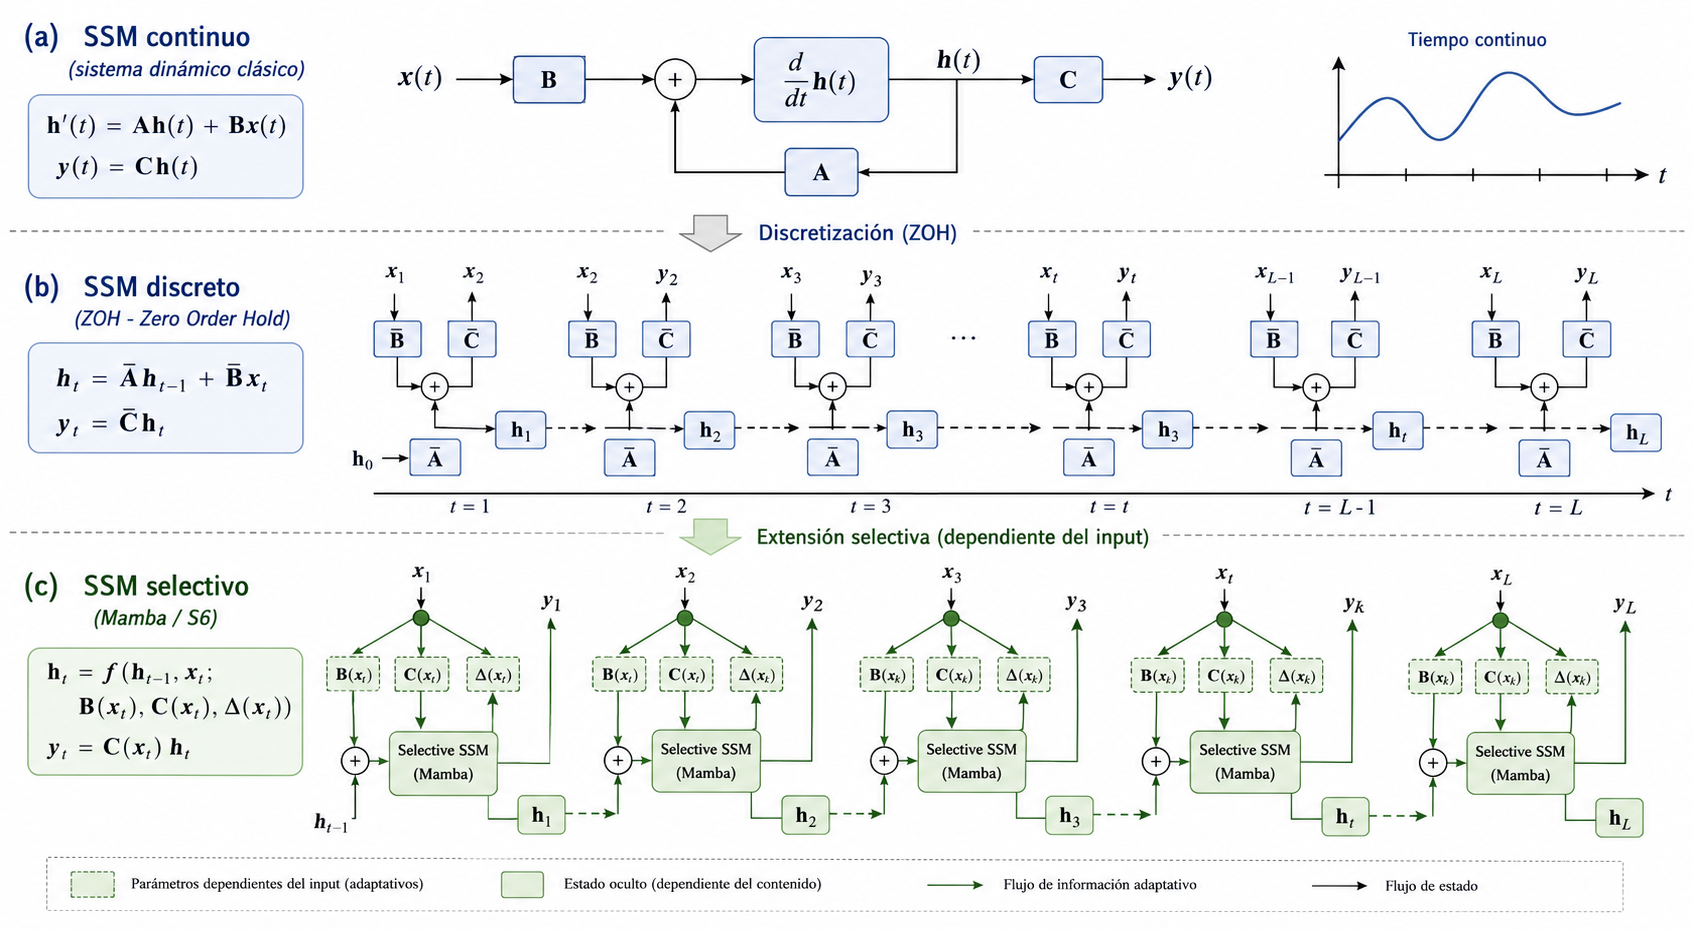
\includegraphics[width=\textwidth]{./images/image9.png}
\caption{Evolución del SSM — lineal, discreto y selectivo (Mamba).}
\label{fig:figure9}
\end{figure}

\subsubsection{Vision Mamba (Vim-Tiny)}

Vision Mamba (Vim) \cite{zhu2024vision} adapta los SSMs selectivos al dominio de la visión
por computadora introduciendo un bloque SSM bidireccional sobre la secuencia de parches de
imagen. La imagen de entrada se tokeniza de la misma forma que en ViT, generando una secuencia
de $N$ tokens. Cada bloque Vim procesa la secuencia en dos direcciones —de izquierda a derecha
y de derecha a izquierda— y fusiona las salidas para producir representaciones bidireccionales,
capturando dependencias tanto causales como anti-causales en la secuencia espacial de parches.

Vim-Tiny, la variante utilizada en esta investigación, cuenta con aproximadamente 7 millones de
parámetros y emplea LayerNorm de forma nativa al inicio de cada bloque, lo que lo sitúa en la
misma categoría de normalización que ViT-Tiny desde la perspectiva de la estabilidad federada.
No obstante, su mecanismo de integración de la información es cualitativamente distinto al de
los ViTs: mientras que la autoatención establece dependencias globales simultáneas entre todos
los pares de tokens, el SSM integra la información mediante transiciones de estado secuenciales
cuya sensibilidad a cada token de entrada depende de la magnitud de $\Delta$ calculado a partir
de ese token \cite{zhu2024vision}. Bajo distribuciones de clases locales distintas entre
clientes, los parámetros SSM —especialmente las proyecciones para $\mathbf{B}$, $\mathbf{C}$ y
$\Delta$— pueden especializarse en secuencias locales representativas de las clases locales,
generando un perfil de drift potencialmente distinto al de ViT \cite{wu2024mamba}.

Desde la perspectiva del rendimiento en dominios médicos, Lai et al.\ \cite{lai2025advancing}
demostraron la competitividad de Vision Mamba en clasificación de tumores cerebrales mediante
\textit{transfer learning}, obteniendo resultados comparables a EfficientNet y ViT. Bansal et
al.\ \cite{bansal2024comprehensive} confirman esta competitividad en múltiples modalidades de
imagen médica. Sin embargo, el comportamiento de Vim-Tiny en el contexto del FL con datos
non-IID y su perfil de drift por capa permanecen sin caracterizar en la literatura existente.


\begin{figure}[ht]
\centering
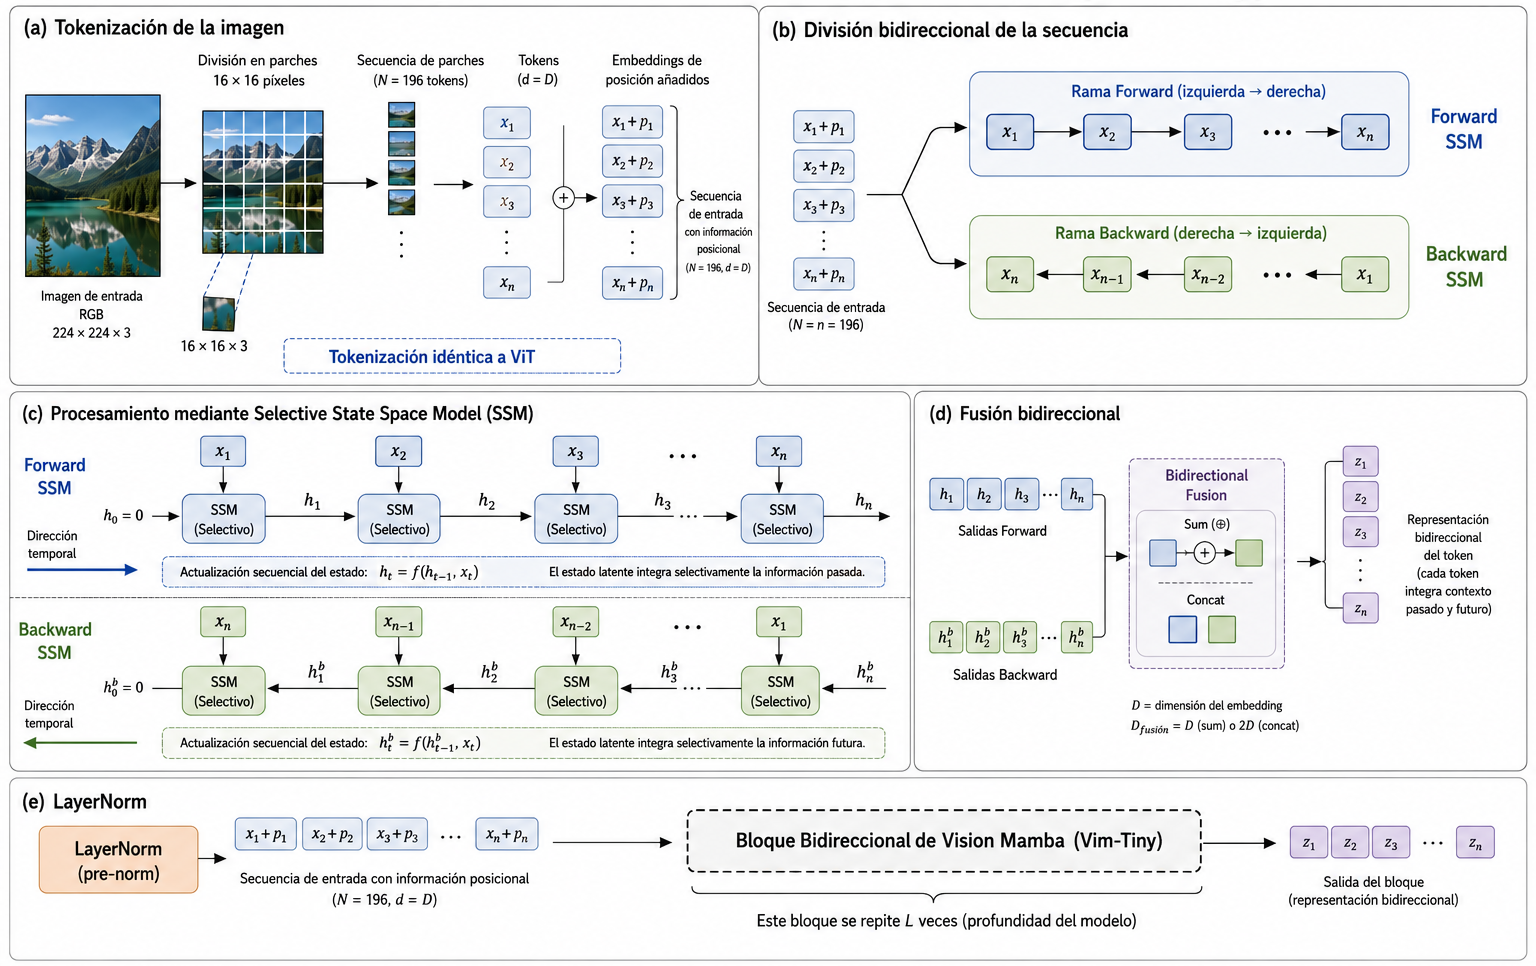
\includegraphics[width=\textwidth]{./images/image10.png}
\caption{Bloque bidireccional de Vision Mamba (Vim).}
\label{fig:figure10}


\end{figure}

\subsection{Vision Graph Neural Networks}

\subsubsection{Graph Neural Networks: propagación de mensajes}

Las redes neuronales en grafos (GNN, \textit{Graph Neural Networks}) son una clase de modelos
de aprendizaje profundo diseñados para operar sobre datos con estructura de grafo
\cite{Scarselli:2009ku}. Un grafo se define como $\mathcal{G} = (\mathcal{V}, \mathcal{E})$,
donde $\mathcal{V} = \{v_1, \ldots, v_n\}$ es el conjunto de nodos y $\mathcal{E} \subseteq
\mathcal{V} \times \mathcal{V}$ es el conjunto de aristas. Cada nodo $v$ posee una
representación vectorial $\mathbf{h}_v^{(l)} \in \mathbb{R}^d$ en la capa $l$, que se actualiza
mediante un proceso de \textit{propagación de mensajes} sobre el vecindario local
$\mathcal{N}(v)$ del nodo:

\begin{equation}
  \mathbf{h}_v^{(l+1)} = \text{UPDATE}\!\left(
    \mathbf{h}_v^{(l)},\;
    \text{AGGREGATE}\!\left(\left\{\mathbf{h}_u^{(l)} : u \in \mathcal{N}(v)\right\}\right)
  \right),
  \label{eq:mpnn}
\end{equation}

donde AGGREGATE es una función permutation-invariante —típicamente suma, media o máximo— y
UPDATE combina la representación actual del nodo con la información agregada de sus vecinos
\cite{Scarselli:2009ku}. El proceso se repite por $L$ capas, permitiendo que cada nodo integre
información de su vecindario de orden $L$.

La propiedad diferenciadora de las GNNs respecto a las CNNs y los ViTs es que la topología
de conectividad —quién es vecino de quién— puede ser dinámica y dependiente del contenido:
las aristas $\mathcal{E}$ no son una restricción estructural fija (como en las CNNs, donde el
vecindario es siempre el parche $k \times k$ adyacente) ni una conectividad completa (como en
los ViTs, donde todos los tokens se atienden mutuamente), sino que pueden construirse
dinámicamente a partir de medidas de similitud en el espacio de representaciones
\cite{senior2023graph, han2022vision}.


\begin{figure}[ht]
\centering
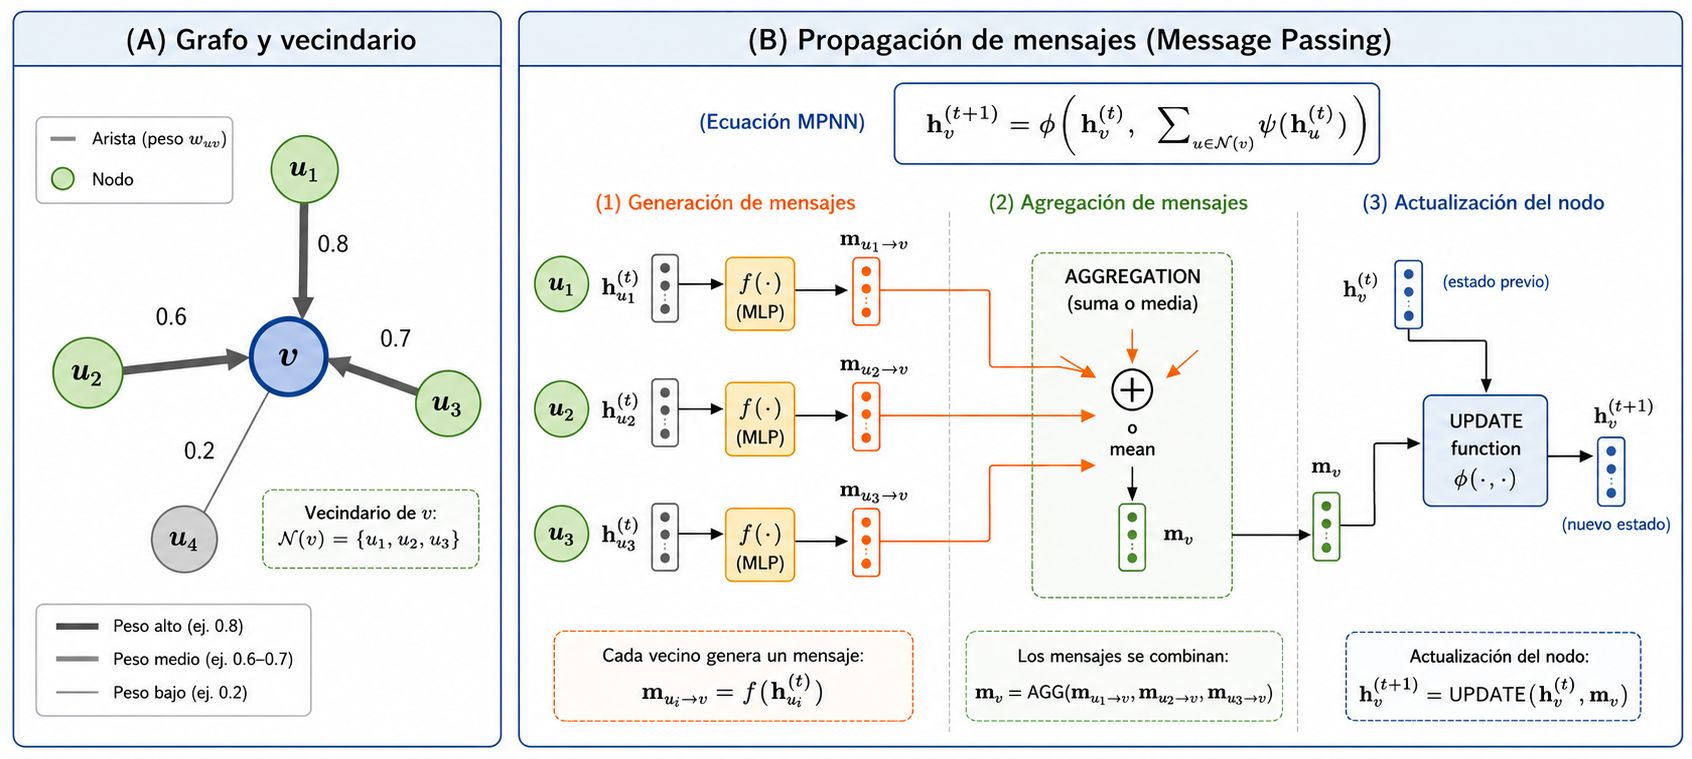
\includegraphics[width=\textwidth]{./images/image11.png}
\caption{Propagación de mensajes en una Graph Neural Network.}
\label{fig:figure11}


\end{figure}


\subsubsection{Vision GNN (ViG-Tiny)}

Han et al.\ \cite{han2022vision} introdujeron Vision GNN (ViG), la primera arquitectura de
visión pura basada en grafos diseñada para clasificación de imágenes a escala de ImageNet.
La arquitectura trata la imagen como un grafo dinámico: los nodos son parches de la imagen,
y las aristas se construyen mediante un grafo $k$-NN (\textit{k-Nearest Neighbors}) en el
espacio de representaciones aprendidas —los $k$ parches más similares en el espacio de
features se conectan mediante aristas dirigidas. Este grafo se reconstruye en cada bloque
a medida que las representaciones evolucionan durante el forward pass, haciendo que la
topología de conectividad sea adaptativa al contenido de la imagen \cite{han2022vision}.

El bloque central de ViG es el \textit{Grapher}, que implementa una operación GNN sobre el
grafo dinámico construido en ese bloque, seguido de un módulo FFN (\textit{Feed-Forward
Network}) análogo al de los ViTs:

\begin{equation}
  \mathbf{H}^{(l+1)} = \text{FFN}\!\left(\text{GNN}\!\left(\mathbf{H}^{(l)},
  \mathcal{G}^{(l)}\right)\right),
  \label{eq:vig_block}
\end{equation}

donde $\mathcal{G}^{(l)}$ es el grafo $k$-NN construido a partir de $\mathbf{H}^{(l)}$
\cite{han2022vision}. La variante ViG-Tiny cuenta con aproximadamente 8 millones de
parámetros y opera sobre imágenes de $224 \times 224$ píxeles, con resolución de tokens
comparable a ViT-Tiny.

El sesgo inductivo de ViG es cualitativamente distinto al de las otras tres familias: la
localidad de las CNNs es espacial y fija; la globalidad de los ViTs es completa y uniforme;
la secuencialidad de los SSMs es lineal y selectiva; la conectividad de ViG es dinámica y
basada en similitud de contenido. Bajo distribuciones de clases locales distintas, el grafo
$k$-NN construido por cada cliente tenderá a conectar parches visualmente similares según las
clases predominantes en sus datos locales, lo que puede introducir patrones de especialización
del Grapher cualitativamente distintos a los de los mecanismos de atención o SSM
\cite{liu2024federated}. La caracterización de este comportamiento en entornos federados
heterogéneos es una de las contribuciones originales de la presente investigación.

Han et al.\ \cite{han2022vision} reportaron resultados competitivos en ImageNet-1K, con ViG-Tiny
superando a DeiT-Tiny en precisión \textit{top-1}. La viabilidad de ViG en entornos federados
fue explorada por primera vez por Cui et al.\ \cite{cui2025fedvig} mediante FedVIG, aunque sin
análisis sistemático de heterogeneidad ni métricas de drift por capa. El presente trabajo
extiende esta línea al entorno experimental controlado de esta investigación.


\begin{figure}[ht]
\centering
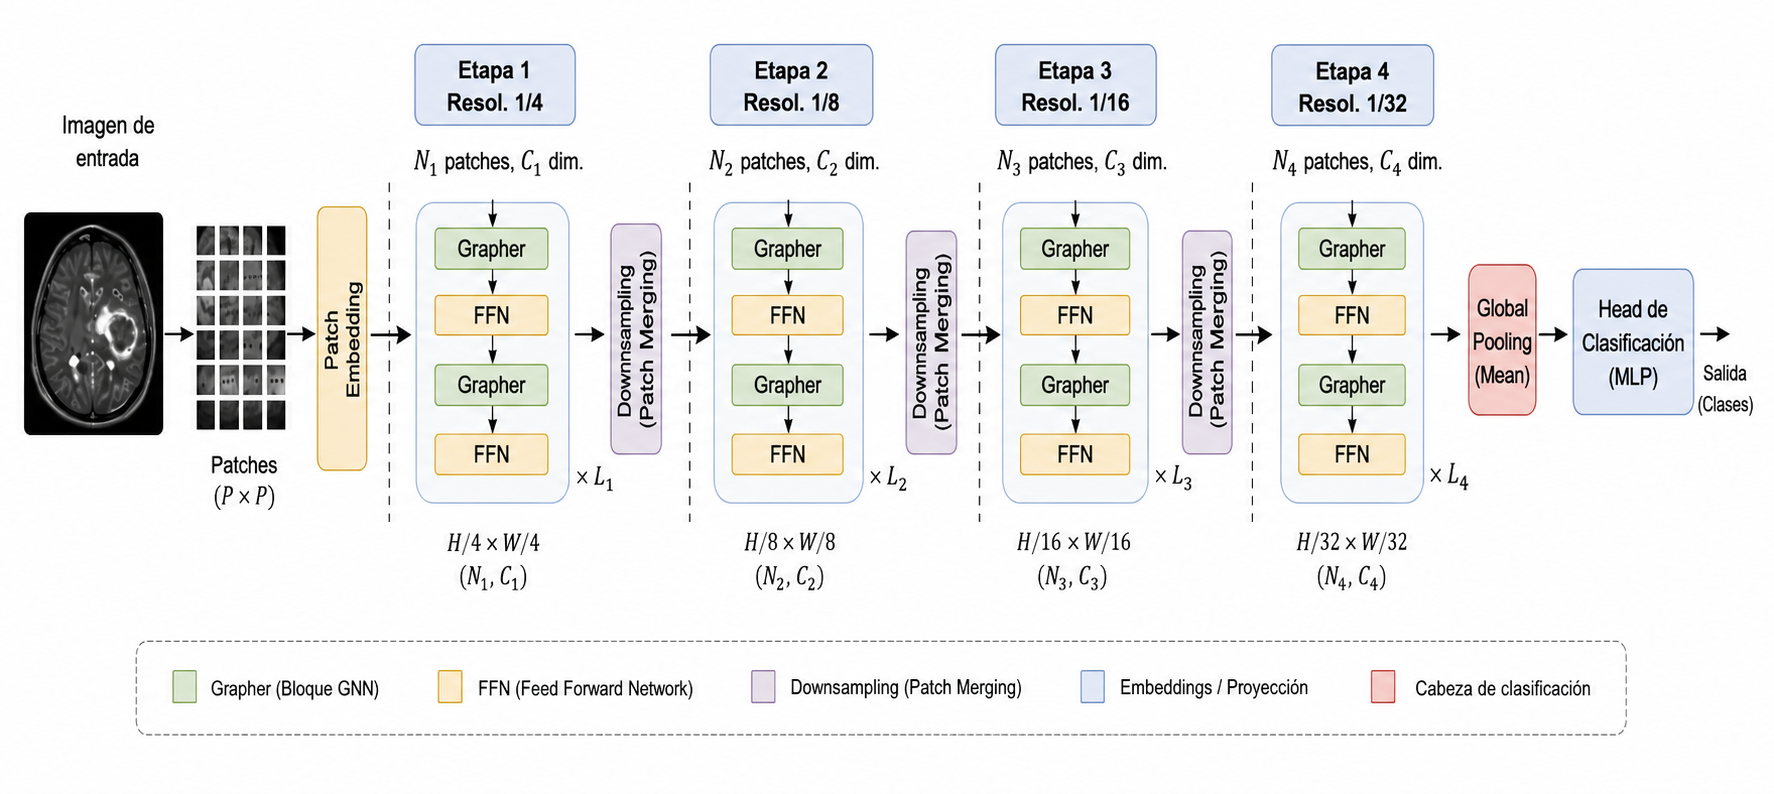
\includegraphics[width=\textwidth]{./images/image12.png}
\caption{Arquitectura de Arquitectura ViG-Tiny.}
\label{fig:figure12}


\end{figure}


\subsection{Estrategias de normalización y sus propiedades en FL}
\label{subsec:normalizacion}

Las distintas estrategias de normalización descritas en las secciones anteriores se diferencian
fundamentalmente por el subconjunto de dimensiones sobre el que calculan las estadísticas de
media y varianza. Esta diferencia determina directamente su estabilidad en entornos federados
con datos heterogéneos \cite{wang2023batch, du2022rethinking, casella2023experimentingnormalizationlayersfederated}.

\textbf{Batch Normalization} (BN) \cite{DBLP:journals/corr/IoffeS15}: normaliza
sobre la dimensión del batch y las dimensiones espaciales, manteniendo estadísticas separadas
por canal. Las estadísticas $\hat{\mu}_{\mathcal{B}}$ y $\hat{\sigma}^2_{\mathcal{B}}$ se
calculan sobre todas las muestras del mini-batch. En FL, estas estadísticas son locales al
cliente y no representan la distribución global, introduciendo el sesgo de gradiente descrito
en la Sección 2.4.1.3 \cite{wang2023batch}.

\textbf{Group Normalization} (GN) \cite{DBLP:journals/corr/abs-1803-08494}: propuesta por Wu
y He, divide los canales de activación en $G$ grupos y normaliza dentro de cada grupo de forma
independiente para cada muestra. Para una activación $\mathbf{x} \in \mathbb{R}^{C \times H
\times W}$, GN calcula:

\begin{equation}
  \mu_{k,g} = \frac{1}{|\mathcal{S}_{k,g}|}\sum_{i \in \mathcal{S}_{k,g}} x_i, \qquad
  \sigma^2_{k,g} = \frac{1}{|\mathcal{S}_{k,g}|}\sum_{i \in \mathcal{S}_{k,g}}
  (x_i - \mu_{k,g})^2,
  \label{eq:gn}
\end{equation}

donde $\mathcal{S}_{k,g}$ es el conjunto de índices del grupo $g$ para la muestra $k$, con
$C/G$ canales por grupo. GN con $G = 1$ es equivalente a Layer Normalization; GN con $G = C$
es equivalente a Instance Normalization. Dado que las estadísticas se calculan por muestra y
por grupo, GN es completamente independiente de la distribución del batch y, en consecuencia,
estable en entornos federados con datos heterogéneos \cite{DBLP:journals/corr/abs-1803-08494,
casella2023experimentingnormalizationlayersfederated}.

La motivación de la ablación de normalización de esta investigación se deriva directamente de
esta taxonomía: al sustituir la BN de EfficientNet-B1 por GN-32 (32 grupos) y por LN
(equivalente a GN-1), se obtienen dos variantes que
conservan exactamente el mismo sesgo inductivo convolucional pero eliminan la dependencia de estadísticas
de mini-batch. Si el
perfil de drift de estas variantes se aproxima al de ViT-Tiny y Vim-Tiny, se concluye que BN
es el factor dominante en la inestabilidad federada de las CNNs; si persisten diferencias
significativas, el sesgo inductivo convolucional tiene una contribución independiente
\cite{pieri2023handlingdataheterogeneityarchitectural, siomos2024architecture}.

% ============================================================
% 2.5 MÉTRICAS DE ANÁLISIS DEL CLIENT DRIFT
% ============================================================
\section{M\'etricas de An\'alisis del Client Drift}

Para caracterizar el client drift con la granularidad requerida por los objetivos de esta
investigación, se necesitan métricas que operen en tres niveles complementarios y no
redundantes: (1) la \textit{divergencia de parámetros}, que cuantifica cuánto se alejan los
pesos del modelo de cada cliente del modelo global en términos de magnitud; (2) la
\textit{alineación de gradientes}, que determina si las actualizaciones de distintos clientes
son constructivas o destructivas entre sí en términos de dirección; y (3) la
\textit{divergencia representacional funcional}, que evalúa si el drift paramétrico implica
o no una divergencia en las representaciones que el modelo aprende a generar. Las tres métricas
empleadas en esta investigación cubren uno de esos niveles cada una, y son complementarias:
sus combinaciones permiten diagnósticos que ninguna métrica individual puede proporcionar de
forma aislada.

\subsection{Divergencia de pesos por capa (\texorpdfstring{$L_2$}{L2} drift)}

La métrica más directa para cuantificar el client drift es la norma $L_2$ de la diferencia
entre los parámetros del modelo local de un cliente y los parámetros del modelo global,
calculada de forma separada para cada capa. Para el cliente $k$, la capa $\ell$ y la ronda de
comunicación $t$, la divergencia de pesos se define como:

\begin{equation}
  \text{drift}_k^{(\ell)}(t) = \left\| \mathbf{w}_k^{(\ell)}(t) -
  \mathbf{w}_{\text{global}}^{(\ell)}(t) \right\|_2,
  \label{eq:l2drift}
\end{equation}

donde $\mathbf{w}_k^{(\ell)}(t)$ son los parámetros de la capa $\ell$ del cliente $k$
inmediatamente antes de la agregación de la ronda $t$, y $\mathbf{w}_{\text{global}}^{(\ell)}(t)$
son los parámetros correspondientes del modelo global al inicio de esa misma ronda. Esta métrica
es la operacionalización directa del pseudo-gradiente definido en la ecuación \eqref{eq:drift},
calculada a nivel de capa en lugar de para el modelo completo \cite{son2022comparisons}.

La estratificación por tipo de capa es fundamental para la interpretabilidad de los resultados.
En esta investigación, los parámetros de cada arquitectura se clasifican en tres grupos
taxonómicos:

\begin{itemize}
  \item \textbf{norm}: capas de normalización (BN, GN o LN según la arquitectura y variante).
  \item \textbf{feature}: capas de extracción de características (bloques MBConv en
    EfficientNet, bloques de atención y MLP en ViT-Tiny, bloques SSM en Vim-Tiny, bloques
    Grapher en ViG-Tiny).
  \item \textbf{head}: la capa clasificadora final (proyección lineal sobre el vector de clase).
\end{itemize}

Son et al.\ \cite{son2022comparisons} establecieron empíricamente que las capas de
clasificación (\textit{head}) exhiben drift sistemáticamente mayor que las capas de extracción
de características de bajo nivel, y que las capas de normalización son las más sensibles a la
heterogeneidad cuando se usa BN. Esta taxonomía permite comparaciones significativas entre
familias arquitectónicas a pesar de que la noción de ``capa de características'' no es
directamente equiparable entre CNNs, ViTs, SSMs y GNNs \cite{son2022comparisons}.

\subsection{Alineación de gradientes entre clientes (similitud coseno)}

La norma $L_2$ del drift cuantifica la magnitud de la divergencia pero no informa sobre si las
actualizaciones de distintos clientes son compatibles entre sí. Dos clientes pueden presentar
alta magnitud de drift pero apuntar en la misma dirección (actualizaciones constructivas) o en
direcciones opuestas (actualizaciones destructivas para la agregación). Para distinguir estos
casos, se emplea la similitud coseno entre los pseudo-gradientes de pares de clientes,
calculada por capa.

Para los clientes $i$ y $j$, la capa $\ell$ y la ronda $t$, la similitud coseno se define como:

\begin{equation}
  \text{cos\_sim}_{i,j}^{(\ell)}(t) =
  \frac{\boldsymbol{\delta}_i^{(\ell)}(t) \cdot \boldsymbol{\delta}_j^{(\ell)}(t)}
  {\left\|\boldsymbol{\delta}_i^{(\ell)}(t)\right\|_2
   \left\|\boldsymbol{\delta}_j^{(\ell)}(t)\right\|_2},
  \label{eq:cossim}
\end{equation}

donde $\boldsymbol{\delta}_k^{(\ell)}(t) = \mathbf{w}_k^{(\ell)}(t) -
\mathbf{w}_{\text{global}}^{(\ell)}(t)$ es el pseudo-gradiente del cliente $k$ en la capa
$\ell$. El resultado toma valores en $[-1, 1]$: valores positivos indican que las
actualizaciones apuntan en la misma dirección general (refuerzo mutuo al promediar); valores
negativos indican que apuntan en direcciones opuestas (interferencia destructiva); el valor
cero indica ortogonalidad (sin interacción constructiva ni destructiva). El perfil de
alineación de gradientes de una arquitectura se obtiene promediando la ecuación \eqref{eq:cossim}
sobre todos los pares $(i, j)$ con $i < j$, reportando el resultado por tipo de capa y por
ronda de comunicación.

Esta métrica es complementaria al $L_2$ drift: una arquitectura puede exhibir bajo drift $L_2$
pero alta interferencia (pseudo-gradientes de pequeña magnitud pero orientaciones opuestas), o
alto drift $L_2$ pero buena alineación (grandes actualizaciones en direcciones consistentes).
La combinación de ambas métricas proporciona un diagnóstico más completo del comportamiento de
la optimización federada que cualquiera de las dos por separado \cite{son2022comparisons}.

\subsection{Centered Kernel Alignment (CKA)}

\subsubsection{Similitud de representaciones neurales}

Las métricas $L_2$ y coseno descritas anteriormente operan sobre los parámetros del modelo y
sus diferencias. Sin embargo, dos modelos con parámetros muy distintos pueden aprender
representaciones funcionalmente equivalentes, especialmente si sus espacios de parámetros son relacionados por transformaciones
ortogonales o de escala \cite{DBLP:journals/corr/abs-1905-00414}. Para evaluar si el drift
paramétrico implica una divergencia funcional en las representaciones aprendidas, se requiere
una métrica que opere directamente sobre las activaciones del modelo y que sea invariante a
transformaciones que no cambian la función computada.

El Centered Kernel Alignment (CKA) \cite{DBLP:journals/corr/abs-1905-00414}, propuesto por
Kornblith et al., satisface esta propiedad. Dadas las matrices de activaciones
$\mathbf{X} \in \mathbb{R}^{n \times p}$ e $\mathbf{Y} \in \mathbb{R}^{n \times q}$
obtenidas al evaluar dos modelos (o el mismo modelo en dos momentos distintos) sobre el mismo
conjunto de $n$ muestras, CKA mide si las relaciones de similitud entre pares de muestras son
consistentes entre las dos representaciones.

\subsubsection{Definición formal del CKA lineal}

El CKA lineal se basa en el estimador de Hilbert-Schmidt Independence Criterion (HSIC) para
matrices de Gram centradas. Las matrices de Gram son:

\begin{equation}
  \mathbf{K} = \mathbf{X}\mathbf{X}^\top \in \mathbb{R}^{n \times n}, \qquad
  \mathbf{L} = \mathbf{Y}\mathbf{Y}^\top \in \mathbb{R}^{n \times n},
  \label{eq:gram}
\end{equation}

y el estimador HSIC centrado es:

\begin{equation}
  \widehat{\text{HSIC}}(\mathbf{K}, \mathbf{L}) =
  \frac{1}{(n-1)^2} \operatorname{tr}(\mathbf{K}\mathbf{H}\mathbf{L}\mathbf{H}),
  \label{eq:hsic}
\end{equation}

donde $\mathbf{H} = \mathbf{I}_n - \frac{1}{n}\mathbf{1}\mathbf{1}^\top$ es la matriz de
centrado. El CKA lineal se define como:

\begin{equation}
  \text{CKA}(\mathbf{X}, \mathbf{Y}) =
  \frac{\widehat{\text{HSIC}}(\mathbf{K}, \mathbf{L})}
  {\sqrt{\widehat{\text{HSIC}}(\mathbf{K}, \mathbf{K})\,
         \widehat{\text{HSIC}}(\mathbf{L}, \mathbf{L})}}.
  \label{eq:cka}
\end{equation}

\sloppy Kornblith et al.\ \cite{DBLP:journals/corr/abs-1905-00414} demostraron que el CKA lineal
posee las siguientes propiedades: (1) \textit{invarianza a transformaciones ortogonales}:
$\text{CKA}(\mathbf{X}\mathbf{Q}, \mathbf{Y}) = \text{CKA}(\mathbf{X}, \mathbf{Y})$ para
cualquier matriz ortogonal $\mathbf{Q}$; (2) \textit{invarianza a isotropías de escala}:
$\text{CKA}(\alpha\mathbf{X}, \mathbf{Y}) = \text{CKA}(\mathbf{X}, \mathbf{Y})$ para
$\alpha > 0$; (3) \textit{acotación}: $\text{CKA} \in [0, 1]$, con $\text{CKA} = 1$ si y
solo si $\mathbf{X}$ e $\mathbf{Y}$ generan el mismo subespacio de columnas (hasta
transformación ortogonal e isotropía de escala); y (4) \textit{simetría}: $\text{CKA}
(\mathbf{X}, \mathbf{Y}) = \text{CKA}(\mathbf{Y}, \mathbf{X})$.

La invarianza a isotropías de escala es particularmente importante en el contexto federado:
los modelos entrenados de forma independiente por distintos clientes pueden diferir en la
escala de sus activaciones incluso cuando aprenden representaciones funcionalmente equivalentes.
Una métrica no invariante a escala penalizaría estas diferencias de escala como divergencia
funcional, mientras que CKA las ignora correctamente \cite{DBLP:journals/corr/abs-1905-00414}.

\subsection{Taxonomía de capas para el análisis por tipo}

La taxonomía de capas \{norm, feature, head\} introducida en la Sección 2.5.1 requiere una
operacionalización específica para cada arquitectura, dado que los tipos de capas no son
directamente equivalentes entre familias. La siguiente correspondencia se utiliza de forma
consistente en todos los experimentos:

Para \textbf{EfficientNet-B1} (y sus variantes GN y LN): el grupo \textit{norm} comprende
todos los parámetros $\gamma$ y $\beta$ de las capas de normalización (BN, GN-32 o LN según
la variante); el grupo \textit{feature} comprende todos los pesos de los bloques MBConv
(convoluciones \textit{depthwise}, proyecciones puntales y módulos SE); el grupo \textit{head}
comprende la capa de clasificación final.

Para \textbf{ViT-Tiny}: el grupo \textit{norm} comprende los parámetros $\gamma$ y $\beta$
de todas las capas LN; el grupo \textit{feature} comprende los pesos de las proyecciones
$\mathbf{Q}$, $\mathbf{K}$, $\mathbf{V}$, las proyecciones de salida de atención y los
bloques MLP; el grupo \textit{head} comprende la cabeza de clasificación aplicada sobre el
token \texttt{[CLS]}.

Para \textbf{Vim-Tiny}: el grupo \textit{norm} comprende los parámetros de LN; el grupo
\textit{feature} comprende las matrices de proyección SSM ($\mathbf{B}$, $\mathbf{C}$, $\Delta$,
$\bar{\mathbf{A}}$, $\bar{\mathbf{B}}$) y las proyecciones de entrada y salida de cada bloque;
el grupo \textit{head} comprende la capa clasificadora.

Para \textbf{ViG-Tiny}: el grupo \textit{norm} comprende las capas de normalización de los
bloques Grapher y FFN; el grupo \textit{feature} comprende los parámetros de las operaciones
GNN (proyecciones de grafos y bloques FFN); el grupo \textit{head} comprende la capa de
clasificación final.

Esta taxonomía garantiza que las comparaciones de drift entre familias sean semánticamente
coherentes: se compara el drift en las capas que cumplen el mismo rol funcional (normalización,
extracción de características, clasificación) a pesar de implementarlo mediante mecanismos
diferentes \cite{son2022comparisons}.

% ============================================================
% 2.6 MÉTRICAS DE EVALUACIÓN DEL RENDIMIENTO
% ============================================================
\section{M\'etricas de Evaluaci\'on del Rendimiento}

\subsection{Métricas de clasificación}

El rendimiento de clasificación de los modelos se evalúa mediante cuatro métricas estándar
calculadas sobre el conjunto de test global al final de cada ronda de comunicación
\cite{sokolova2009systematic}.

La \textit{accuracy} (exactitud global) mide la proporción de muestras correctamente
clasificadas sobre el total:
$\text{Acc} = \frac{\text{TP} + \text{TN}}{\text{TP} + \text{TN} + \text{FP} + \text{FN}}$,
donde TP, TN, FP y FN son verdaderos positivos, verdaderos negativos, falsos positivos y
falsos negativos, respectivamente.

La \textit{precision} (\textit{precision} macro-promediada) mide la proporción de predicciones
positivas correctas para cada clase, promediada sobre las $C$ clases:
$\text{Precision} = \frac{1}{C}\sum_{c=1}^C \frac{\text{TP}_c}{\text{TP}_c + \text{FP}_c}$.

El \textit{recall} (sensibilidad macro-promediada) mide la proporción de positivos correctamente
identificados por clase:
$\text{Recall} = \frac{1}{C}\sum_{c=1}^C \frac{\text{TP}_c}{\text{TP}_c + \text{FN}_c}$.

El \textit{F1-Score} macro-promediado es la media armónica de precision y recall:
$\text{F1} = \frac{2 \cdot \text{Precision} \cdot \text{Recall}}{\text{Precision} + \text{Recall}}$.

En el dataset Brain Tumor MRI, el F1-score macro es preferible a la accuracy como métrica
principal porque trata cada clase con igual peso, independientemente de su frecuencia en la
partición local de cada cliente: bajo heterogeneidad Dirichlet elevada, un modelo puede
acumular alta accuracy concentrando predicciones en las clases más representadas en su
subconjunto local, mientras que el F1-macro penaliza esa concentración, lo que resulta más
informativo del rendimiento de generalización global y del riesgo clínico asociado a
clasificaciones erróneas de categorías diagnósticas minoritarias en un cliente dado
\cite{noor2026federated, appasami2025federated}.

\subsection{Convergencia y estabilidad}

La convergencia del proceso de aprendizaje federado se evalúa mediante la curva de accuracy o
F1 global a lo largo de las $T$ rondas de comunicación. Una curva que aumenta
monotónicamente y se estabiliza en un plateau indica convergencia estable; oscilaciones
persistentes indican alta varianza inducida por el drift o incompatibilidad entre las
actualizaciones de los clientes.

La estabilidad se cuantifica mediante la desviación estándar de la métrica de rendimiento final
sobre tres semillas de inicialización independientes (42, 123 y 456), reportando los resultados
como $\mu \pm \sigma$. El uso de múltiples semillas es especialmente importante en FL porque el
entrenamiento federado introduce fuentes adicionales de varianza respecto al entrenamiento
centralizado: la partición aleatoria de los datos entre clientes, la selección de clientes por
ronda y la inicialización de los parámetros del modelo \cite{DBLP:journals/corr/abs-1912-04977}.
Una arquitectura con bajo $\sigma$ entre semillas es más predecible y, por tanto, más confiable
para despliegues clínicos o industriales reales.

\subsection{Equidad entre clientes (fairness)}

La equidad federada (\textit{federated fairness}) evalúa si el modelo global entrenado
beneficia de forma homogénea a todos los clientes o si favorece sistemáticamente a los clientes
con distribuciones de datos más representativas de la distribución global
\cite{DBLP:journals/corr/abs-1912-04977}. En esta investigación, la equidad se operacionaliza
como la varianza del F1-score entre clientes al final del entrenamiento:

\begin{equation}
  \text{Fairness}(t) = \text{Var}_{k \in \{1, \ldots, K\}}\!\left[
    F1_k^{(\text{test})}(t)
  \right],
  \label{eq:fairness}
\end{equation}

donde $F1_k^{(\text{test})}(t)$ es el F1-score del modelo global evaluado sobre el conjunto de
test del cliente $k$ en la ronda $t$. Un valor bajo de esta varianza indica que todos los
clientes obtienen rendimiento similar con el modelo global; un valor alto indica que algunos
clientes —típicamente aquellos con distribuciones de clase muy alejadas de la media— se
benefician significativamente menos del entrenamiento colaborativo.

En el dominio médico, la relevancia de la equidad es crítica: un modelo de clasificación de
tumores cerebrales que alcanza alta precisión global pero falla sistemáticamente en los clientes
con alta proporción de casos de meningioma —una clase subrepresentada en la distribución
global— representa un riesgo diagnóstico para los pacientes atendidos en esas instituciones
\cite{noor2026federated}. La medición sistemática de la equidad por arquitectura permitirá
identificar qué familias arquitectónicas producen modelos globales más equitativos bajo
diferentes niveles de heterogeneidad, complementando el análisis de rendimiento promedio con
una dimensión de justicia distributiva.

